\chapter{Data-driven Background Estimation}
\label{cha:datadrivenbg}

One does observe a sizeable contribution from backgrounds like $t\bar{t}$ after the final step of the event selection. This is the case despite them being unable to produce two prompt same sign charge muons. That necessitates the source of at least one of two selected leptons to be some sort of deficiency. Muons from jets or other secondary interactions could be falsely associated with the vertex in question. Another possibility are punch-through particles traversing the HCAL and leaving tracks in the muon system. For example fragments from a hadronic interaction, like a charged pion or kaon, could yield enough hits in the chambers, given enough energy. As a result, this particle may be misidentified as a muon, if a coincidentally matching trajectory can be found in the tracker. Both cases lead to a ``fake muon''. Obviously only the latter is a \textit{true} fake muon, but both occurrences are usually handled simultaneously. The corresponding selection requirements are isolation for the secondary interaction case and the trajectory quality criteria for the punch-through one. However, preventing either scenario from happening by tightening their thresholds is unlikely to impossible. With how difficult simulating these QCD multijet event dominated scenarios can be, the poor agreement between data and prediction can be improved by utilizing an used portion of the measurement. To estimate the contribution of fakes from data, the ``fake rate method'' is employed.


\section{Fake Rate Method}
\label{sec:fakerate}

The fake rate method will replace roughly half of the Monte Carlo samples with the data-driven estimate of QCD contributions. This encompasses the following backgrounds. $W +$ jets, production of single tops, top pairs and top pairs with real photons as well as the entirety of the QCD samples. On the other hand the Drell-Yan processes, two and three vector boson backgrounds, top pair production with additional vector bosons, $W + \gamma$ and rare samples will be taken from simulation.

The general idea of the fake rate method is to estimate fake contributions by comparing one tightly and one loosely selected muon sample. It should be noted that \textit{loose} muons are only selected for this data-driven background estimation, while the ones used in the analysis are denoted as \textit{tight}\footnote{The dimuon criteria are not applied for the data-driven background estimate.} ones. Two criteria are used to split the samples from one another. First and foremost, the combined relative isolation criterion is being raised from $I_{\text{rel}} < 0.12$ to $I_{\text{rel}} < 0.5$. This adds a sizeable contribution from backgrounds such as QCD and $t \bar{t}$ with muons stemming from secondary interactions. Additionally, the transverse impact parameter requirement has been loosened from $d_{xy} < 0.2\,\text{mm}$ to $d_{xy} < 2\,\text{mm}$. Therefore the restrictions on the vertices and as such the threshold for cosmic muons are lowered.

\begin{figure}[ht!]
  \centering
    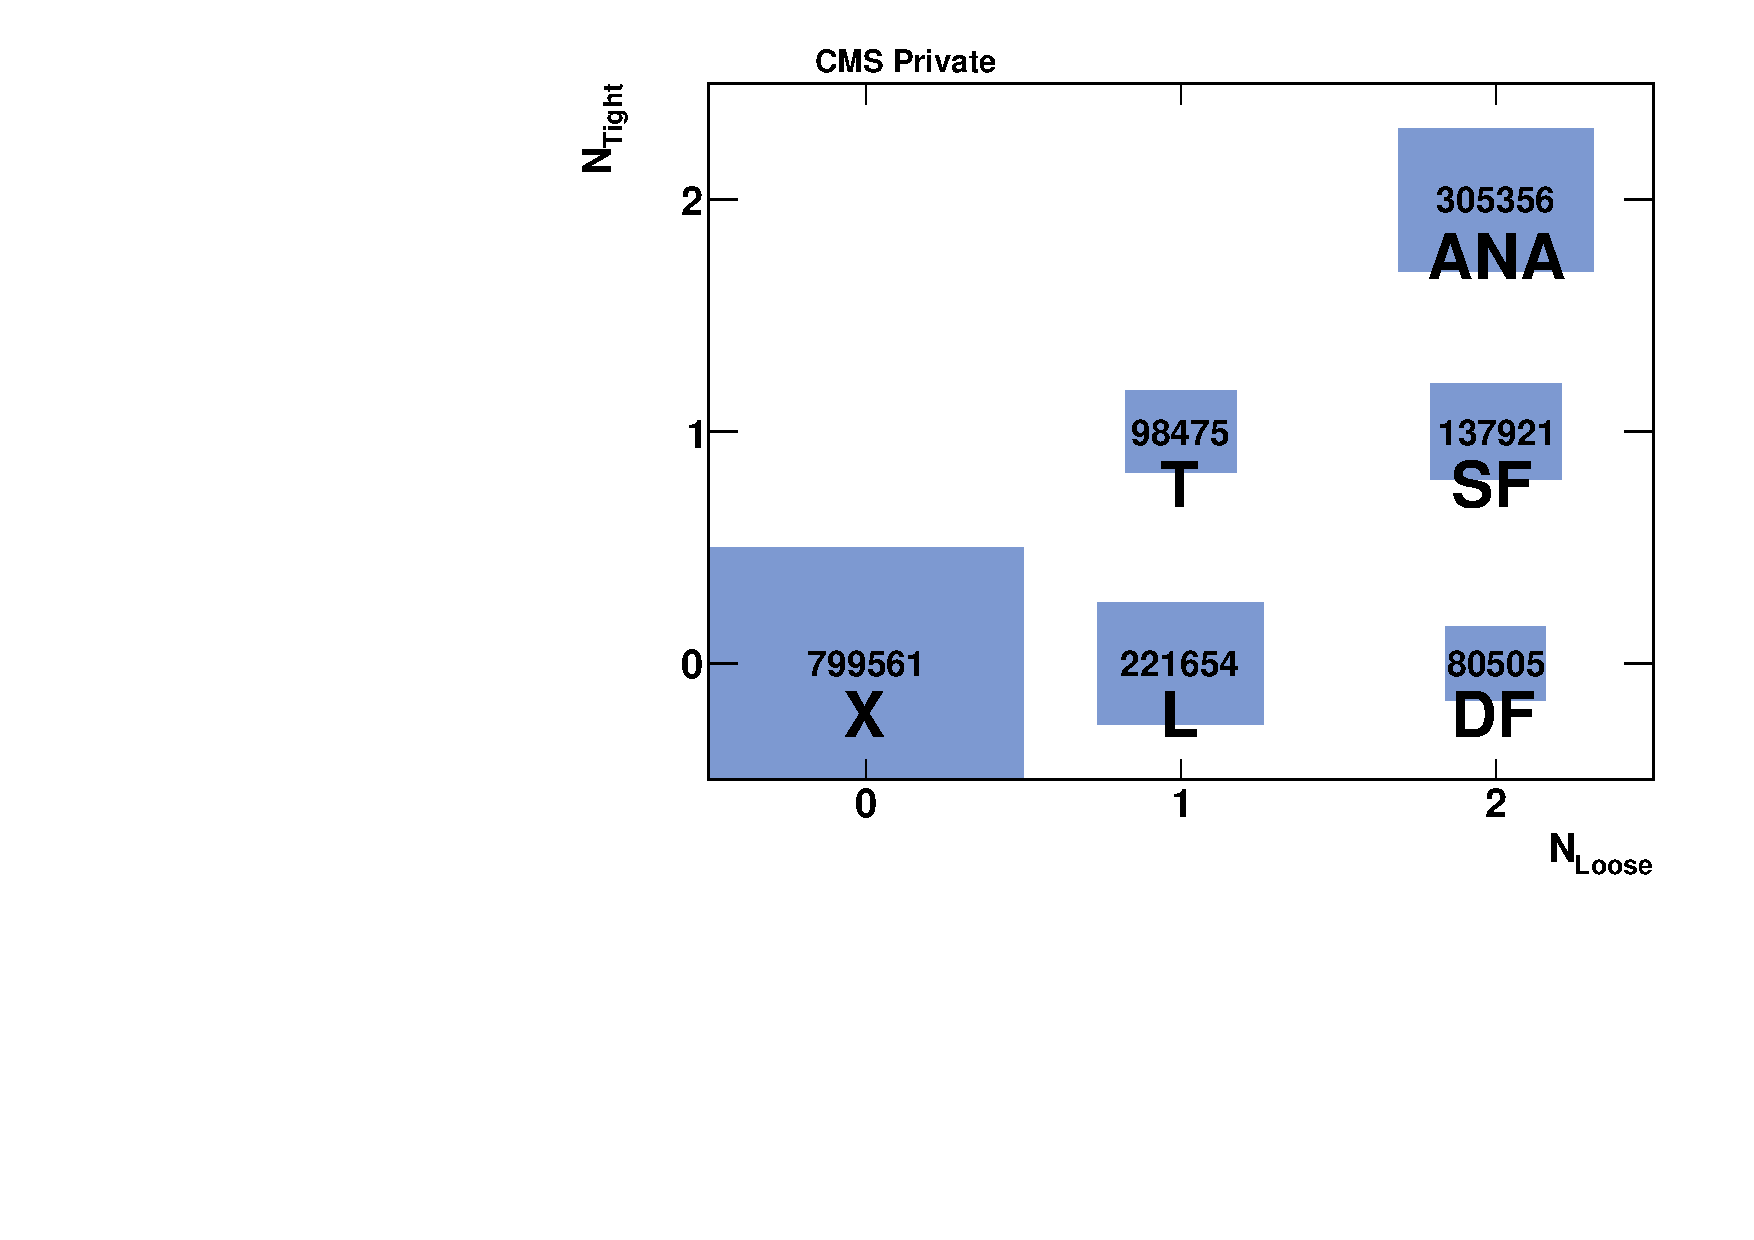
\includegraphics[width=0.6\textwidth]{plots/nloosetight.pdf}
  \caption{Number of loose versus number of tight muons as measured in data. T - Tight, L - Loose, SF - Single-fake, DF - Double-fake, ANA - Analysis sample, X - Not used.}
  \label{fig:nloosetight}
\end{figure}

To measure the fake rate independently from the final distribution, an orthogonal sample needs to be procured. Much like the control regions being defined by an inverted MET requirement, the overall number of loose muons in an event can be used. Here the fraction of tight to loose muons $F_R = \frac{T}{T+L}$\footnote{This is often falsely called the ``fake rate'', thus naming the method.} can be determined (C.f. fig.~\ref{fig:nloosetight}). To account for possible dependencies introduced by the detector, it is measured in both $\eta$ and $p_{\text{T}}$. 

Using $F_R$, the number of tight muons $N_T$ can be predicted from the number of loose ones $N_L$. The definition of loose muons also includes all tight ones. Therefore, to stay in line with the independence of samples, one has to ensure that amongst the number of loose muons $N_L$, there are \textit{no} tight ones. The resulting formula is given below.

\begin{equation}
  \label{eq:fakerate}
  N_T = f \cdot N_L = \frac{F_R }{1 - F_R} \cdot N_L
\end{equation}

When looking for two prompt muons, either one or both of them can be faked. Depending on whether or not the specific background can produce a prompt muon, one of the two cases will be prevalent. For ``single-fakes'', $W +$ jets or top pair production are prime examples. To predict the number of single-fakes from an orthogonal sample, one of the analysis' tight muons is replaced with a loose (but \textit{not} tight) muon (C.f. fig.~\ref{fig:nloosetight}). Summing up the number of events at the desired stage and applying the weight $f$, yields the number of single-fakes $N_{SF}$.

\begin{equation}
  \label{eq:singlefakes}
  N_{SF} = \sum_{tl} f = \sum_{tl} \frac{F_R^1}{1 - F_R^1}
\end{equation}

\noindent The additional index $i$ of the tight-to-loose ratio $F_R^i$ represents the dependency on the transverse momentum and pseudorapidity of the specific muon. 

If both muons are faked, ``double-fakes'', the scenario has to be adjusted. Prime examples for this case are interactions dominated by hadronic activity, primarily the $QCD$ background. Demanding two loose muons (which are \textit{not} tight) serves the purpose of splitting the sample from the analysis' one in this case (C.f. fig.~\ref{fig:nloosetight}). The event weight $f$ is now composed of individual weights $f^i (p_{\text{T}}^j, \eta^j)$ for each of the $j = 1, 2$ muons.

\begin{equation}
  \label{eq:doublefakes}
  N_{DF} = \sum_{ll} f = \sum_{ll} f^1 f^2 = \sum_{ll} \frac{F_R^1}{1 - F_R^1} \cdot \frac{F_R^2}{1 - F_R^2}
\end{equation}

One would naively expect the sum of both cases to be the overall amount of fakes. However, the double-fake scenario is also embedded in the single-fake one. If the tight muon of the latter case has been faked, it becomes the double-fake scenario (Eq.~\ref{eq:doublefakes}). Since either of the two loose leptons of the double-fake case is able to fake the tight one, it is contributing \textit{twice} to the single-fake case (Eq.~\ref{eq:singlefakes}).

\begin{equation}
  \label{eq:fakes}
  N_{fakes} = N_{SF} - N_{DF} =  \sum_{tl} \frac{F_R^1}{1 - F_R^1} - \sum_{ll} \frac{F_R^1}{1 - F_R^1} \cdot \frac{F_R^2}{1 - F_R^2}
\end{equation}


\section{Measurement}
\label{sec:tlmeasurement}

Estimating the background starts off by measuring the tight-to-loose ratio $F_R = \frac{T}{T+L}$. For that, the definition and selection of tight and loose muons is the first step. This is done after the event cleaning (Sec.~\ref{sec:evclean}), but before the basic muon selection (Sec.~\ref{sec:basicmuon}). Therefore events with any number of muons, specifically ones with less than two muons that pass the ID, can be included. For the \textit{tight} subset, almost all of the muon quality criteria (Sec.~\ref{sec:muonqualy}) are applied. The only exceptions are the distance to the next jet and the distance between two muons. These requirements are only meant for selecting the two muons candidates of the analysis. They may otherwise introduce a bias it towards the specific final state, thus limiting the prediction. As already stated before, \textit{loose} muons are defined by the same rules, but only have to abide $I_{\text{rel}} < 0.5$ and $d_{xy} < 2\,\text{mm}$.

Demanding exactly one loose muon (Fig.~\ref{fig:ntlnloose}) yields an independent sample. Since the prediction of fakes is strongly correlated to the amount of QCD multijet events, various kinematic and topologic requirements can be applied to isolate these. Requiring two jets (Fig.~\ref{fig:ntlnjets}) ensures a minimum amount of hadronic activity per event. With each jet's transverse momentum exceeding $50\,\text{GeV}$ (Fig.~\ref{fig:ntljetpt}), the Drell-Yan background is being suppressed. After setting the minimum transverse momentum of the first muon to $20\,\text{GeV}$ and all remaining ones to at least $10\,\text{GeV}$(Fig.~\ref{fig:ntlmupt}), the $Z$-peak can be eliminated for the same purpose. Thus the invariant mass of two muons\footnote{The two muons encompass the one loose muon as well as one muon which passes the ID, but does not qualify as a loose muon.} closest to the $Z$-mass, is restricted to a window from $10\,\text{GeV}$ to $80\,\text{GeV}$ (Fig.~\ref{fig:ntlzmass}). By setting an upper bound of $40\,\text{GeV}$ for the missing transverse energy (Fig.~\ref{fig:ntlmet}), the top-quark and $W$-Boson backgrounds are being discriminated against, as QCD processes generally do not contain a lot of $E_{T}^{miss}$. By using the transverse mass hypothesis for a leptonically decaying $W$ boson, it is also possible to reduce the same backgrounds. Requiring the value of the transverse mass of the loose muon and the missing transverse energy to be less than $40\,\text{GeV}$ (Fig.~\ref{fig:ntlmt}) decreases the contribution of said backgrounds, while passing QCD multijet events. Also, motivating a QCD-like back-to-back topology can be achieved through limiting the azimuth angle between the leading jet and loose muon to $\Delta \phi > 1$ (Fig.~\ref{fig:ntljetdphi}).

In general, one can observe reasonable agreement between data and simulation in the $n - 1$ distributions. In particular in regards to the electroweak processes. However in QCD dominated histograms, there is a noticeable lack of QCD contributions towards higher energies. One major reason are the leading order cross sections used for these samples. Additionally only a fraction of the enormous amount of hadronic activity can be simulated adequately. The large event weights given in table~\ref{tab:mcsamples}, are a testament to that. As a result, the statistics for QCD multijet events are also lacking.

\begin{figure}[b!]
  \centering
  \begin{subfigure}[b]{0.495\textwidth}
    \centering
    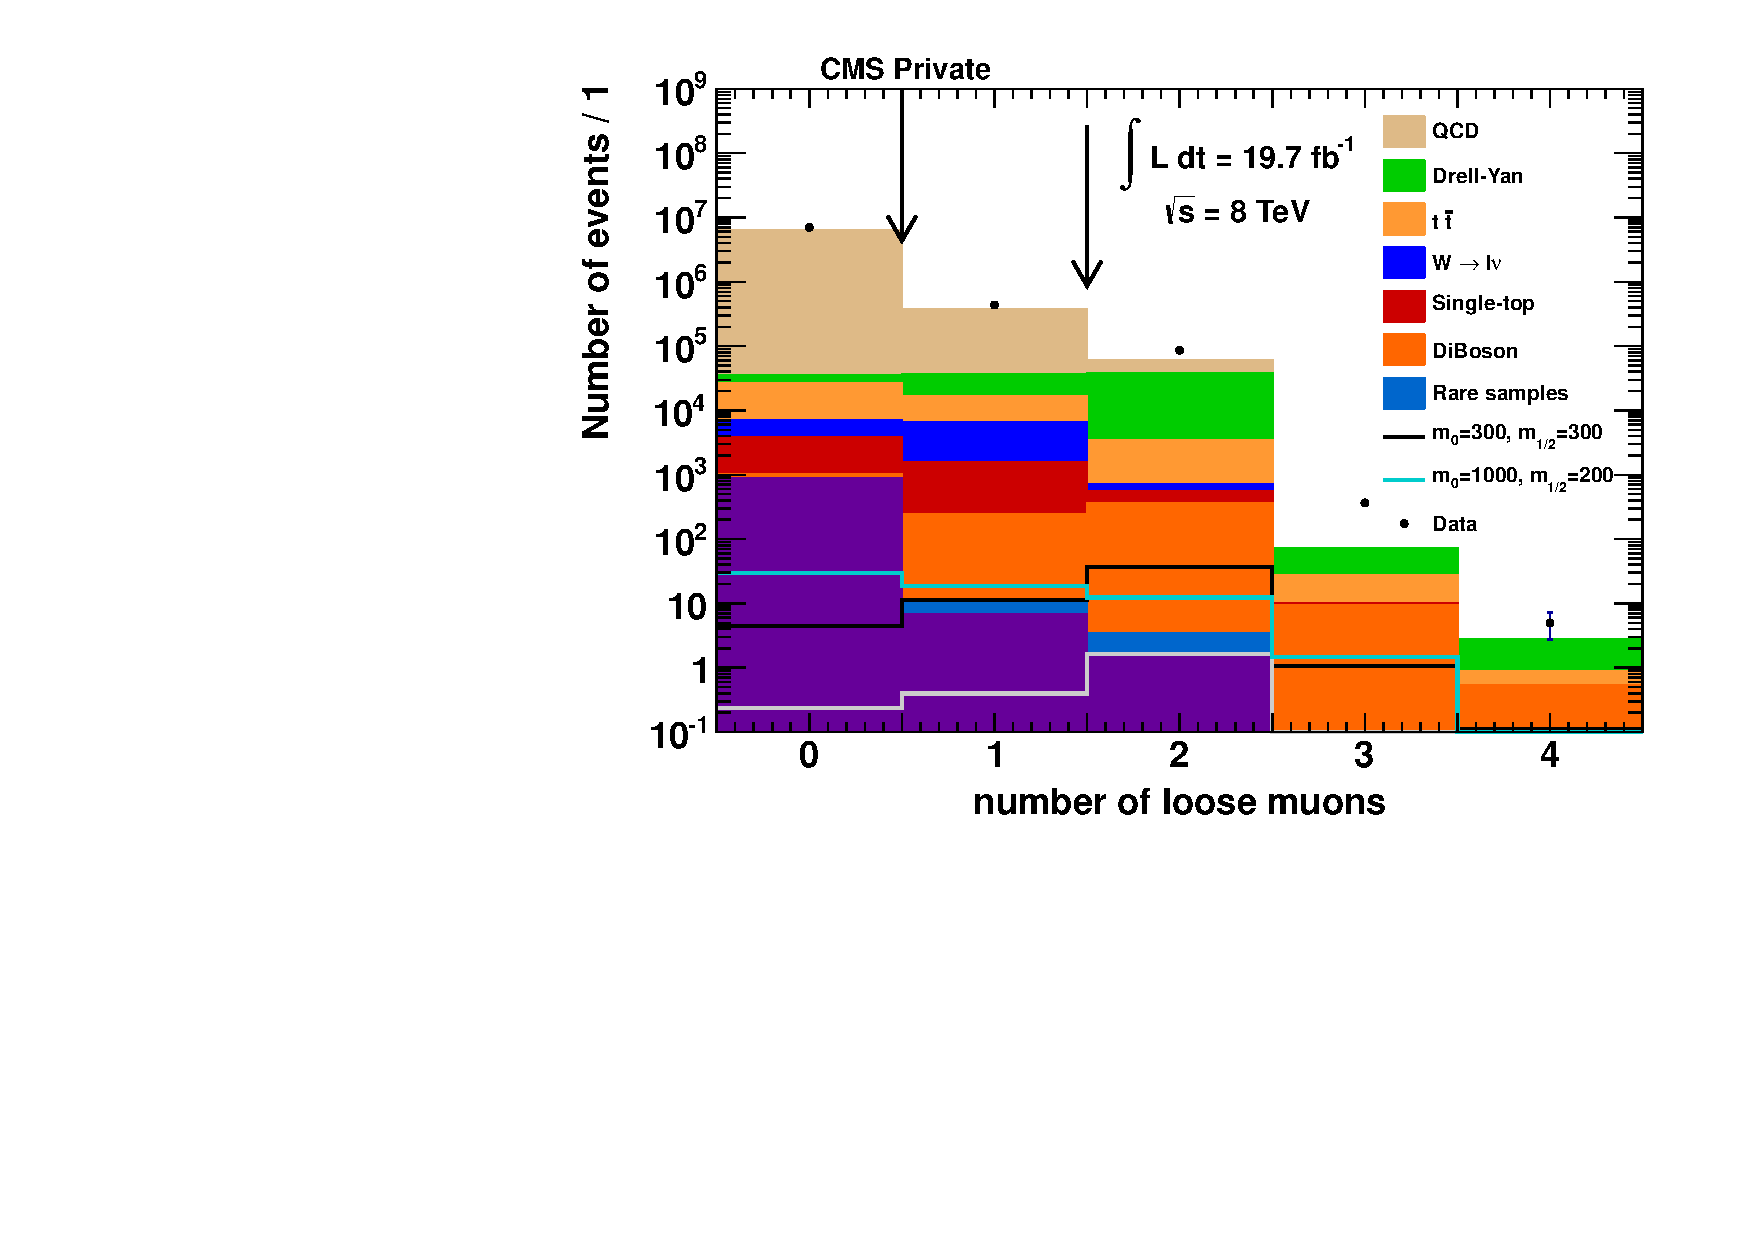
\includegraphics[width=\textwidth]{plots/nTL_nloose.pdf}
    \caption{Number of loose muons\label{fig:ntlnloose}}
  \end{subfigure}
  \begin{subfigure}[b]{0.495\textwidth}
    \centering
    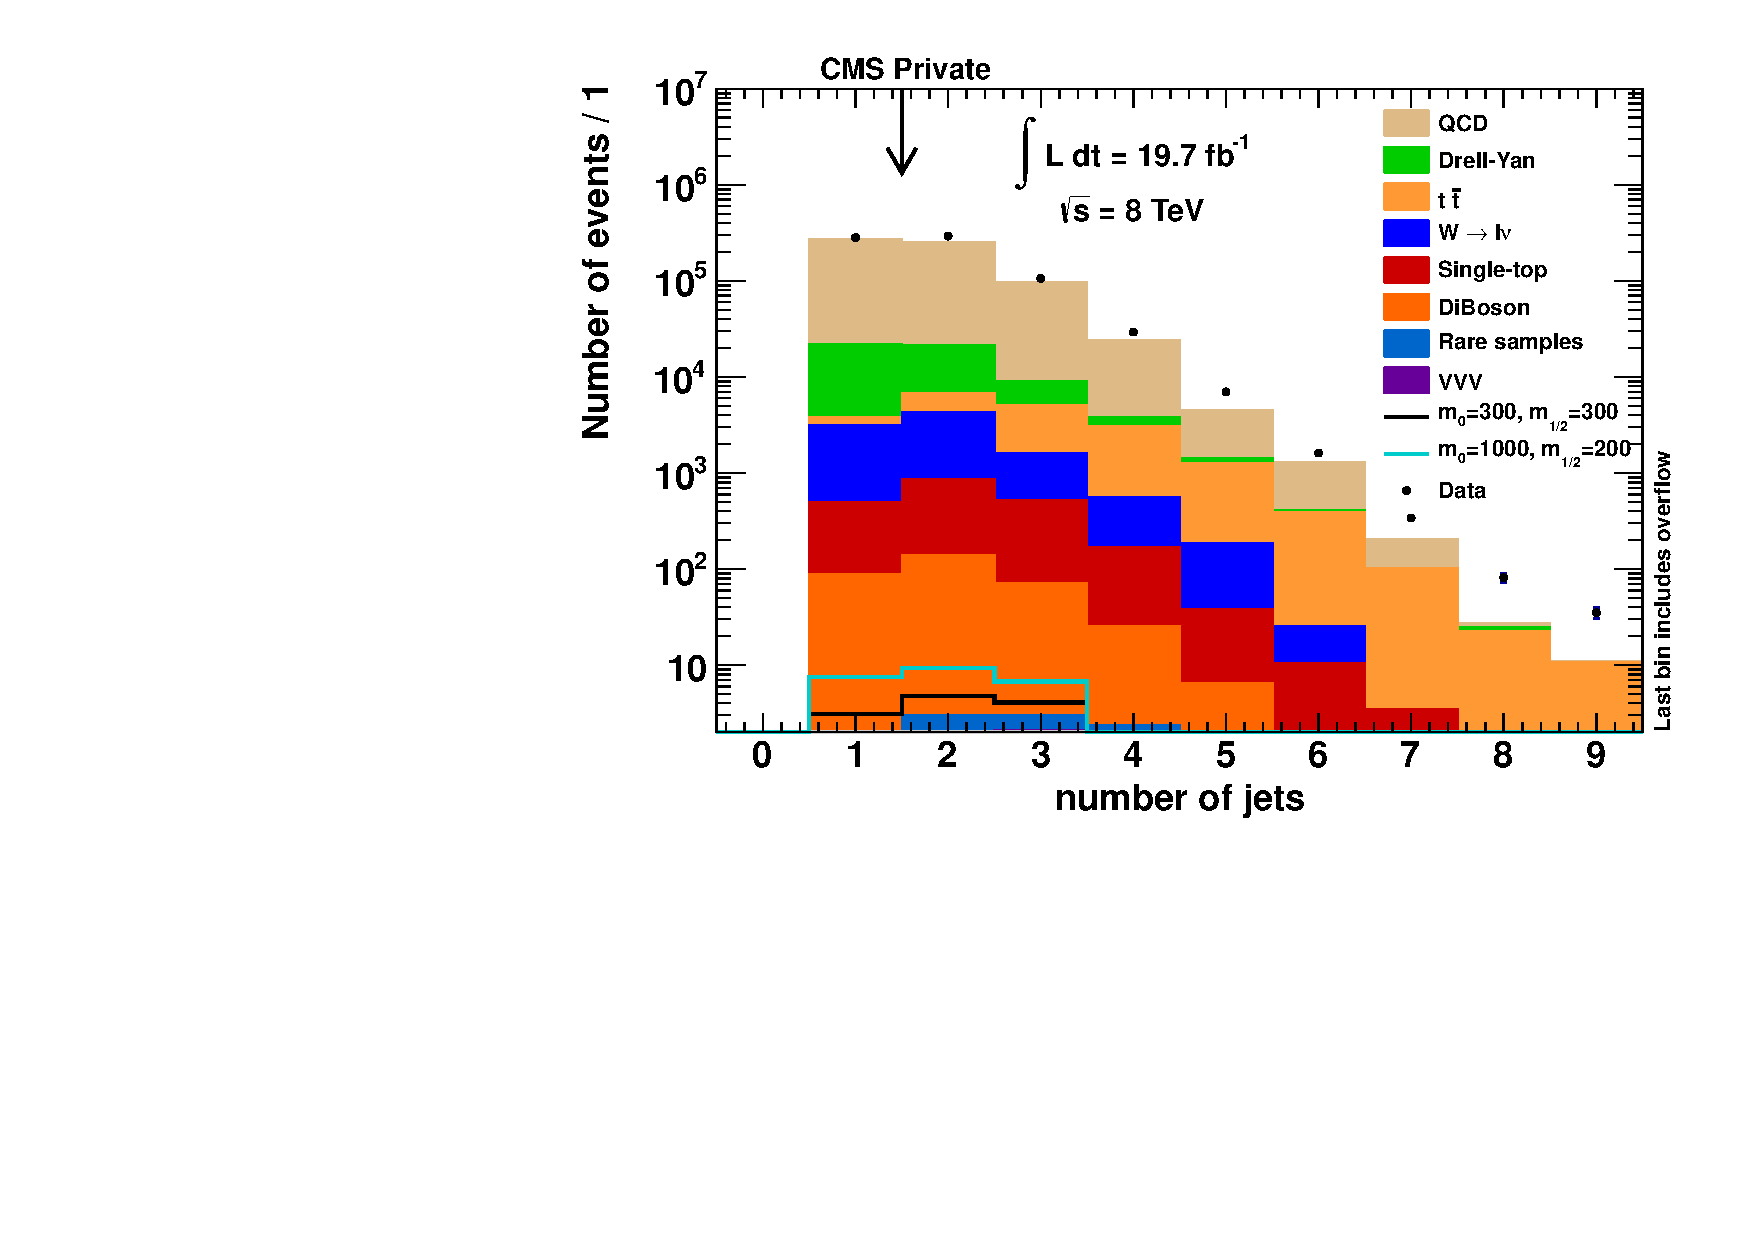
\includegraphics[width=\textwidth]{plots/nTL_njets.pdf}
    \caption{Number of jets\label{fig:ntlnjets}}
  \end{subfigure}
\end{figure}

\begin{figure}[b!]
  \ContinuedFloat
  \centering
  \begin{subfigure}[b]{0.495\textwidth}
    \centering
    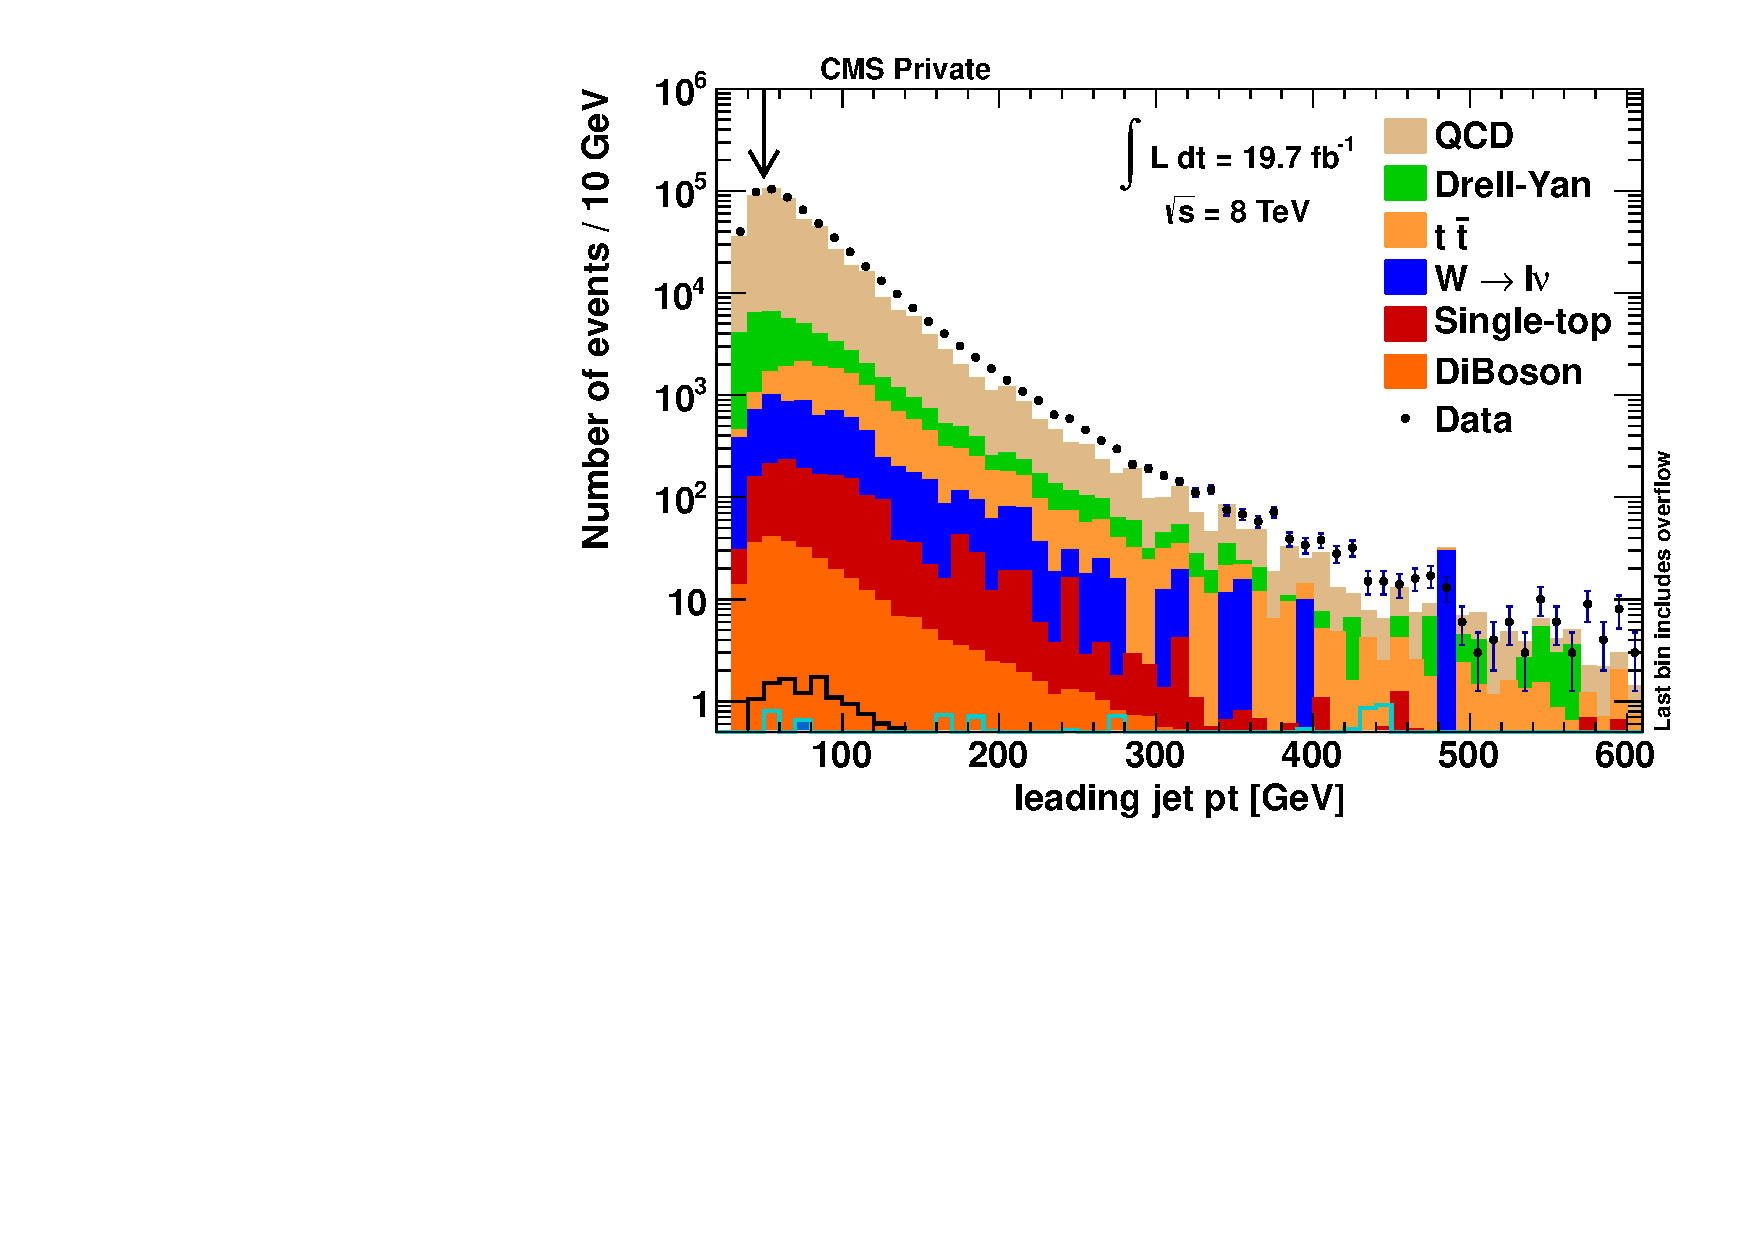
\includegraphics[width=\textwidth]{plots/nTL_jetpt.pdf}
    \caption{Transverse momentum of jets\label{fig:ntljetpt}}
  \end{subfigure}
  \begin{subfigure}[b]{0.495\textwidth}
    \centering
    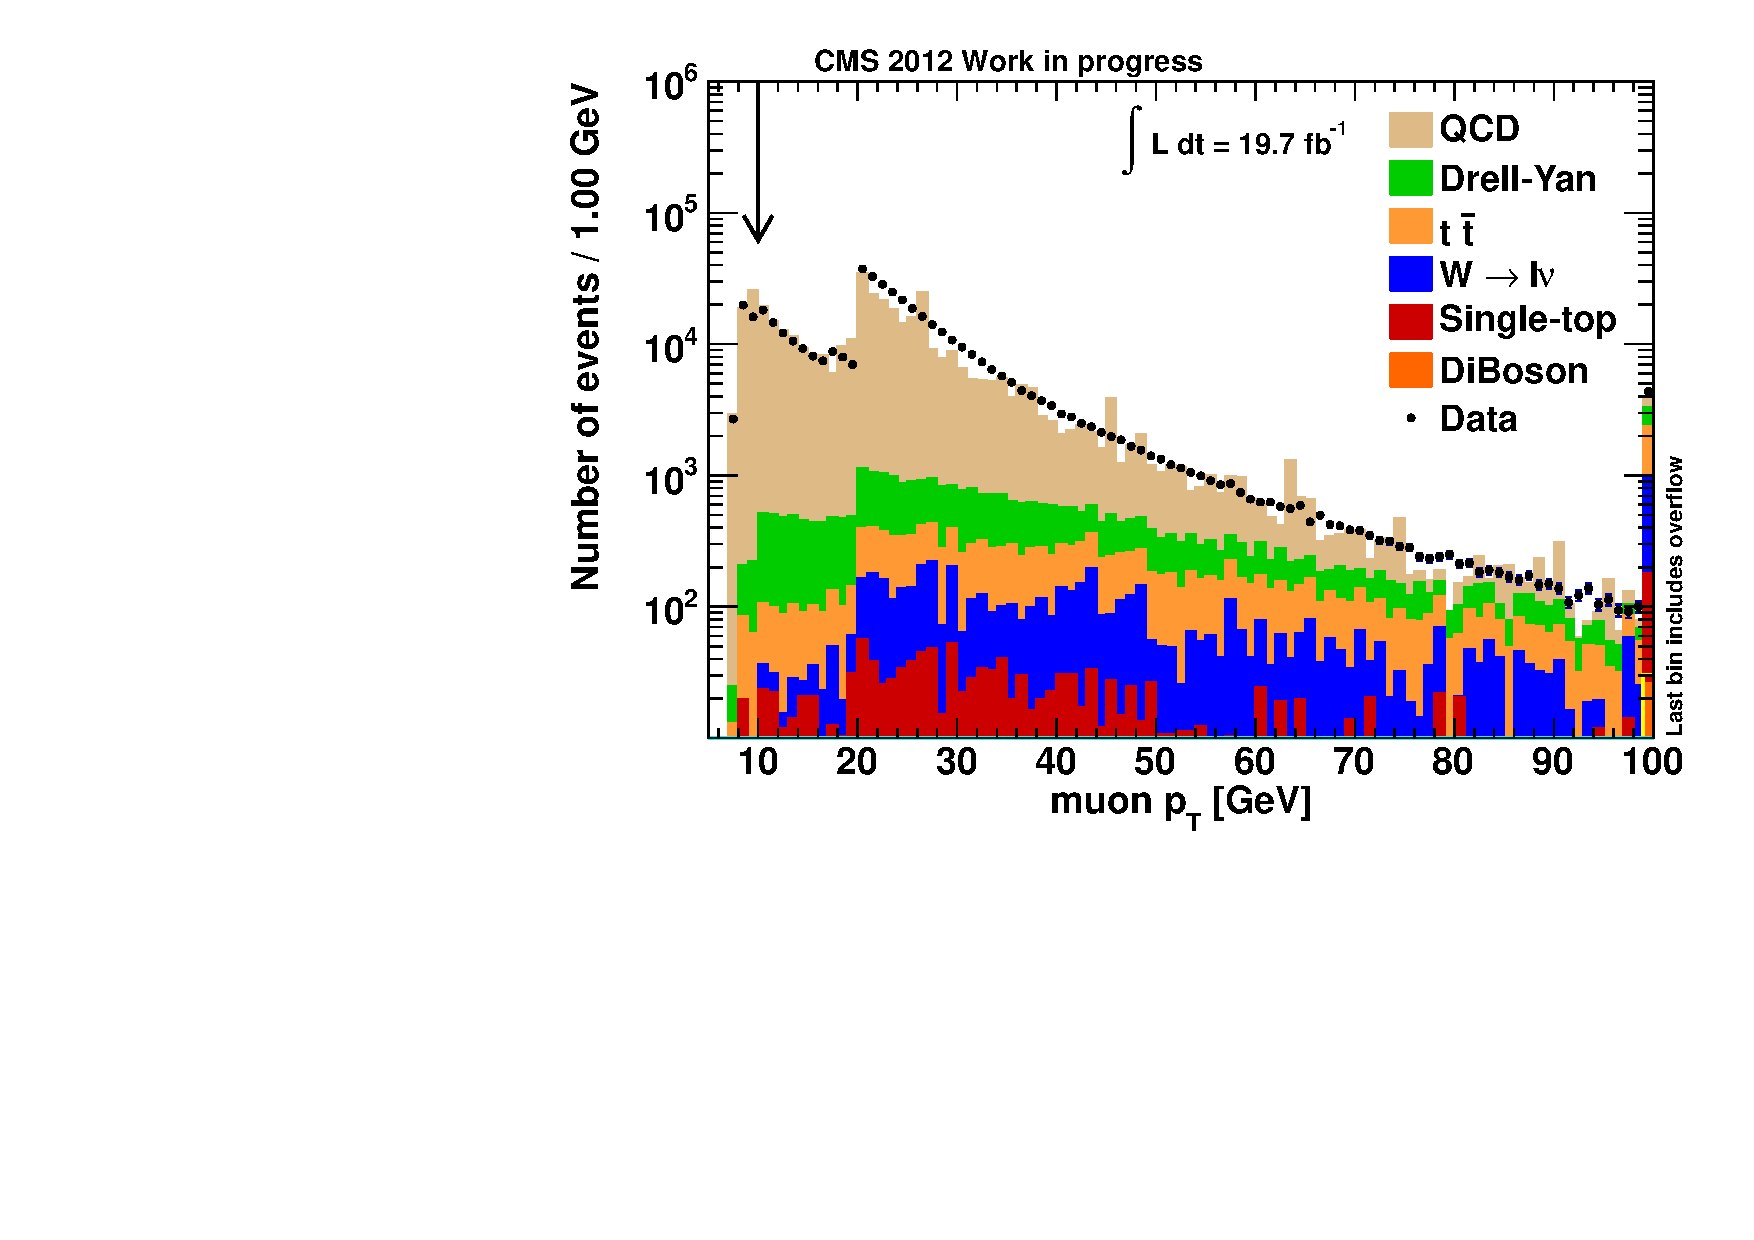
\includegraphics[width=\textwidth]{plots/nTL_mupt.pdf}
    \caption{Transverse momentum of muons \label{fig:ntlmupt}}
  \end{subfigure}
\end{figure}

\begin{figure}[htbp!]
  \ContinuedFloat
  \centering
  \begin{subfigure}[b]{0.495\textwidth}
    \centering
    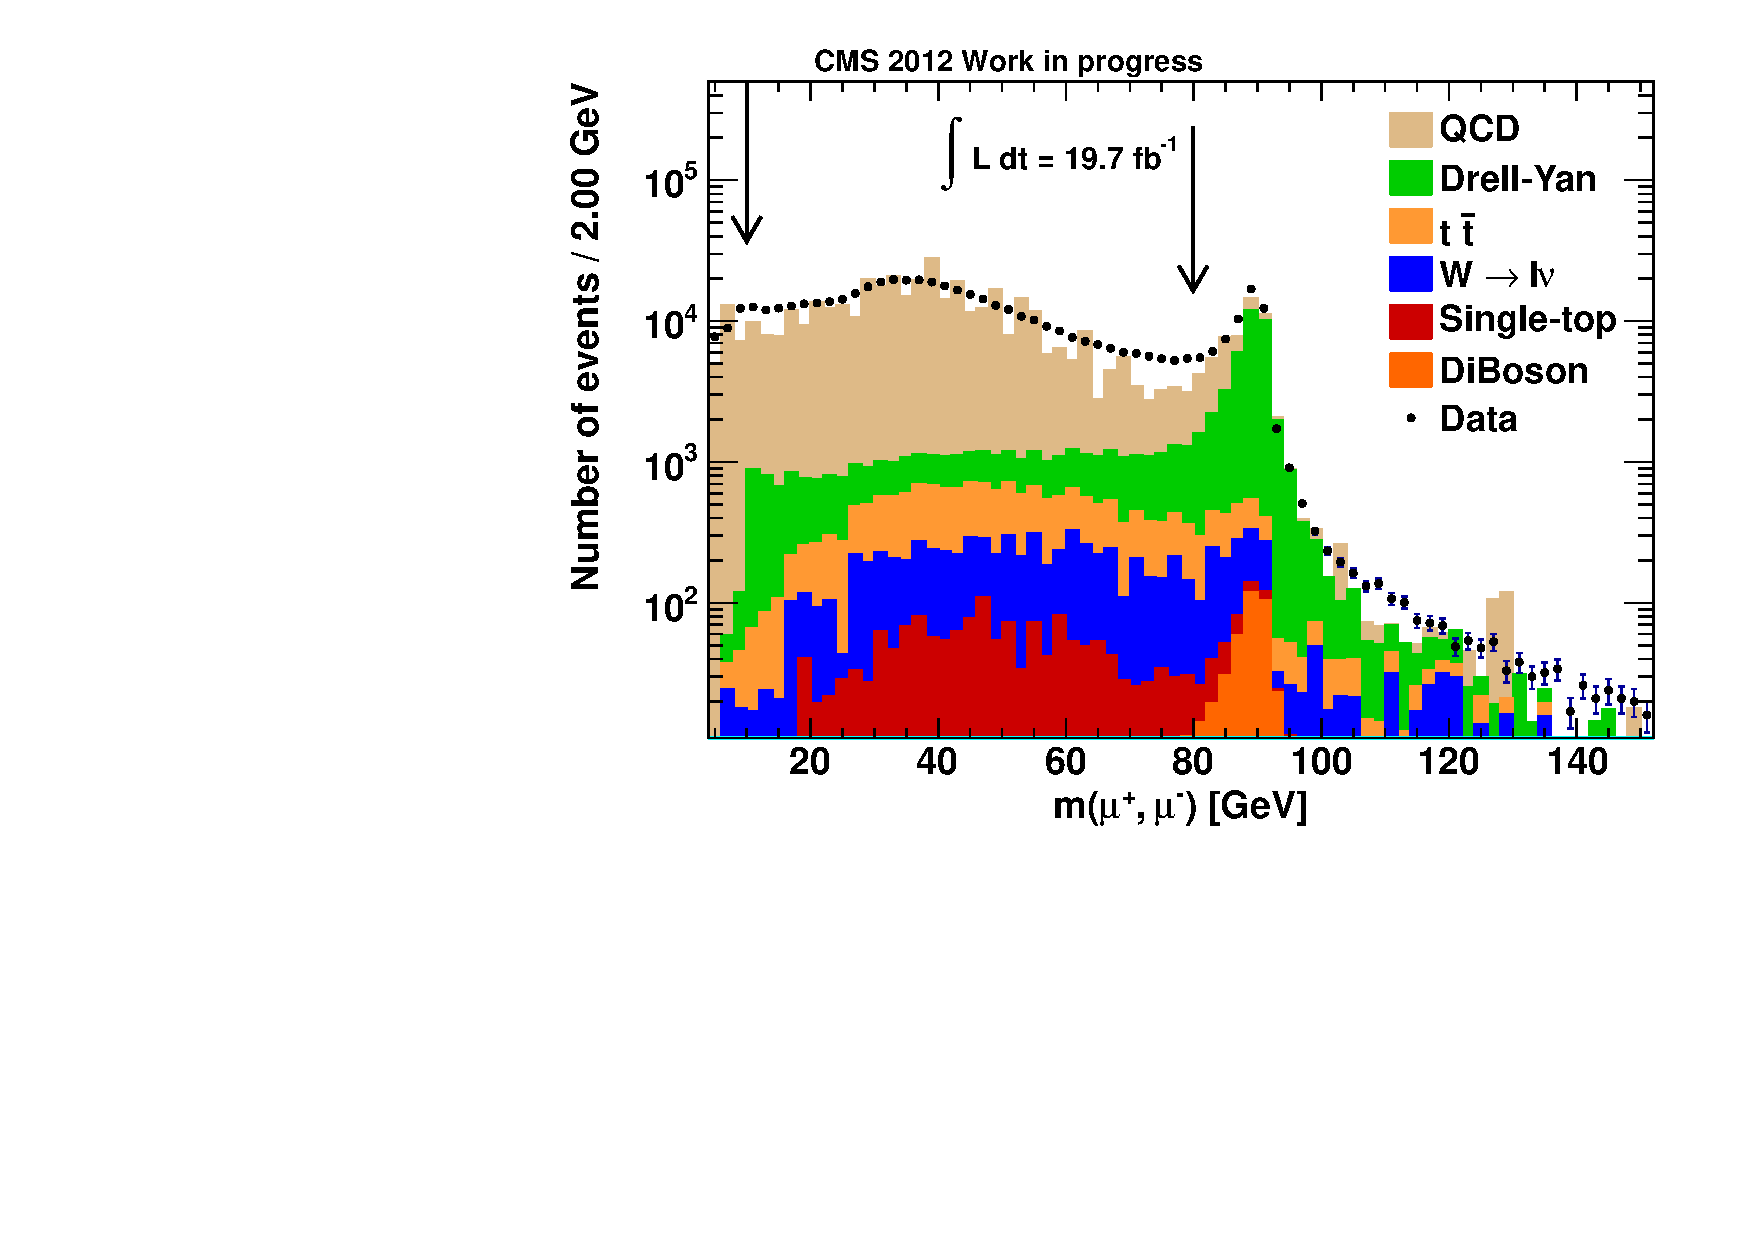
\includegraphics[width=\textwidth]{plots/nTL_zmass.pdf}
    \caption{Invariant dimuon mass closest to $Z$-mass \label{fig:ntlzmass}}
  \end{subfigure}
  \begin{subfigure}[b]{0.495\textwidth}
    \centering
    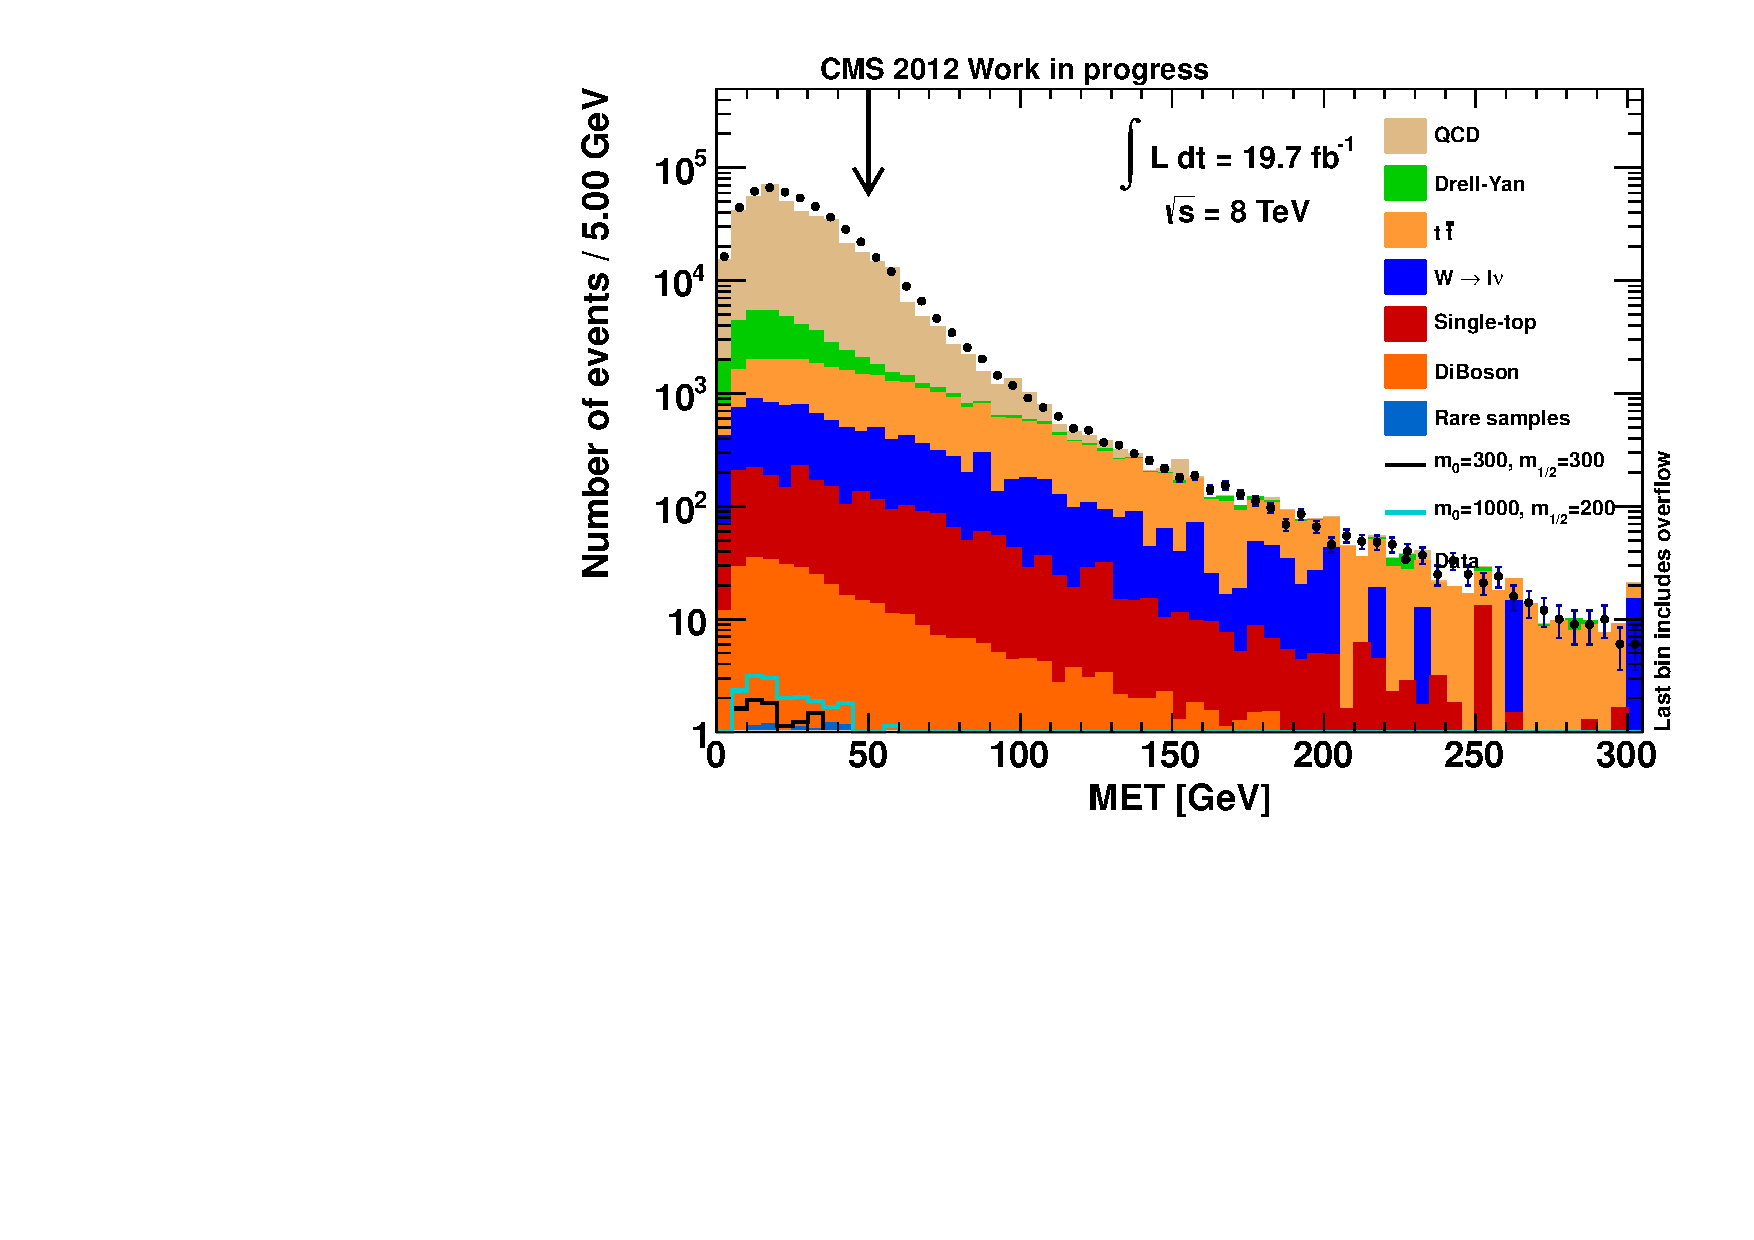
\includegraphics[width=\textwidth]{plots/nTL_met.pdf}
    \caption{Transverse missing energy $E_{\text{T}}^{\text{miss}}$ \label{fig:ntlmet}}
  \end{subfigure}
\end{figure}

\begin{figure}[htbp!]
  \ContinuedFloat
  \centering
  \begin{subfigure}[b]{0.495\textwidth}
    \centering
    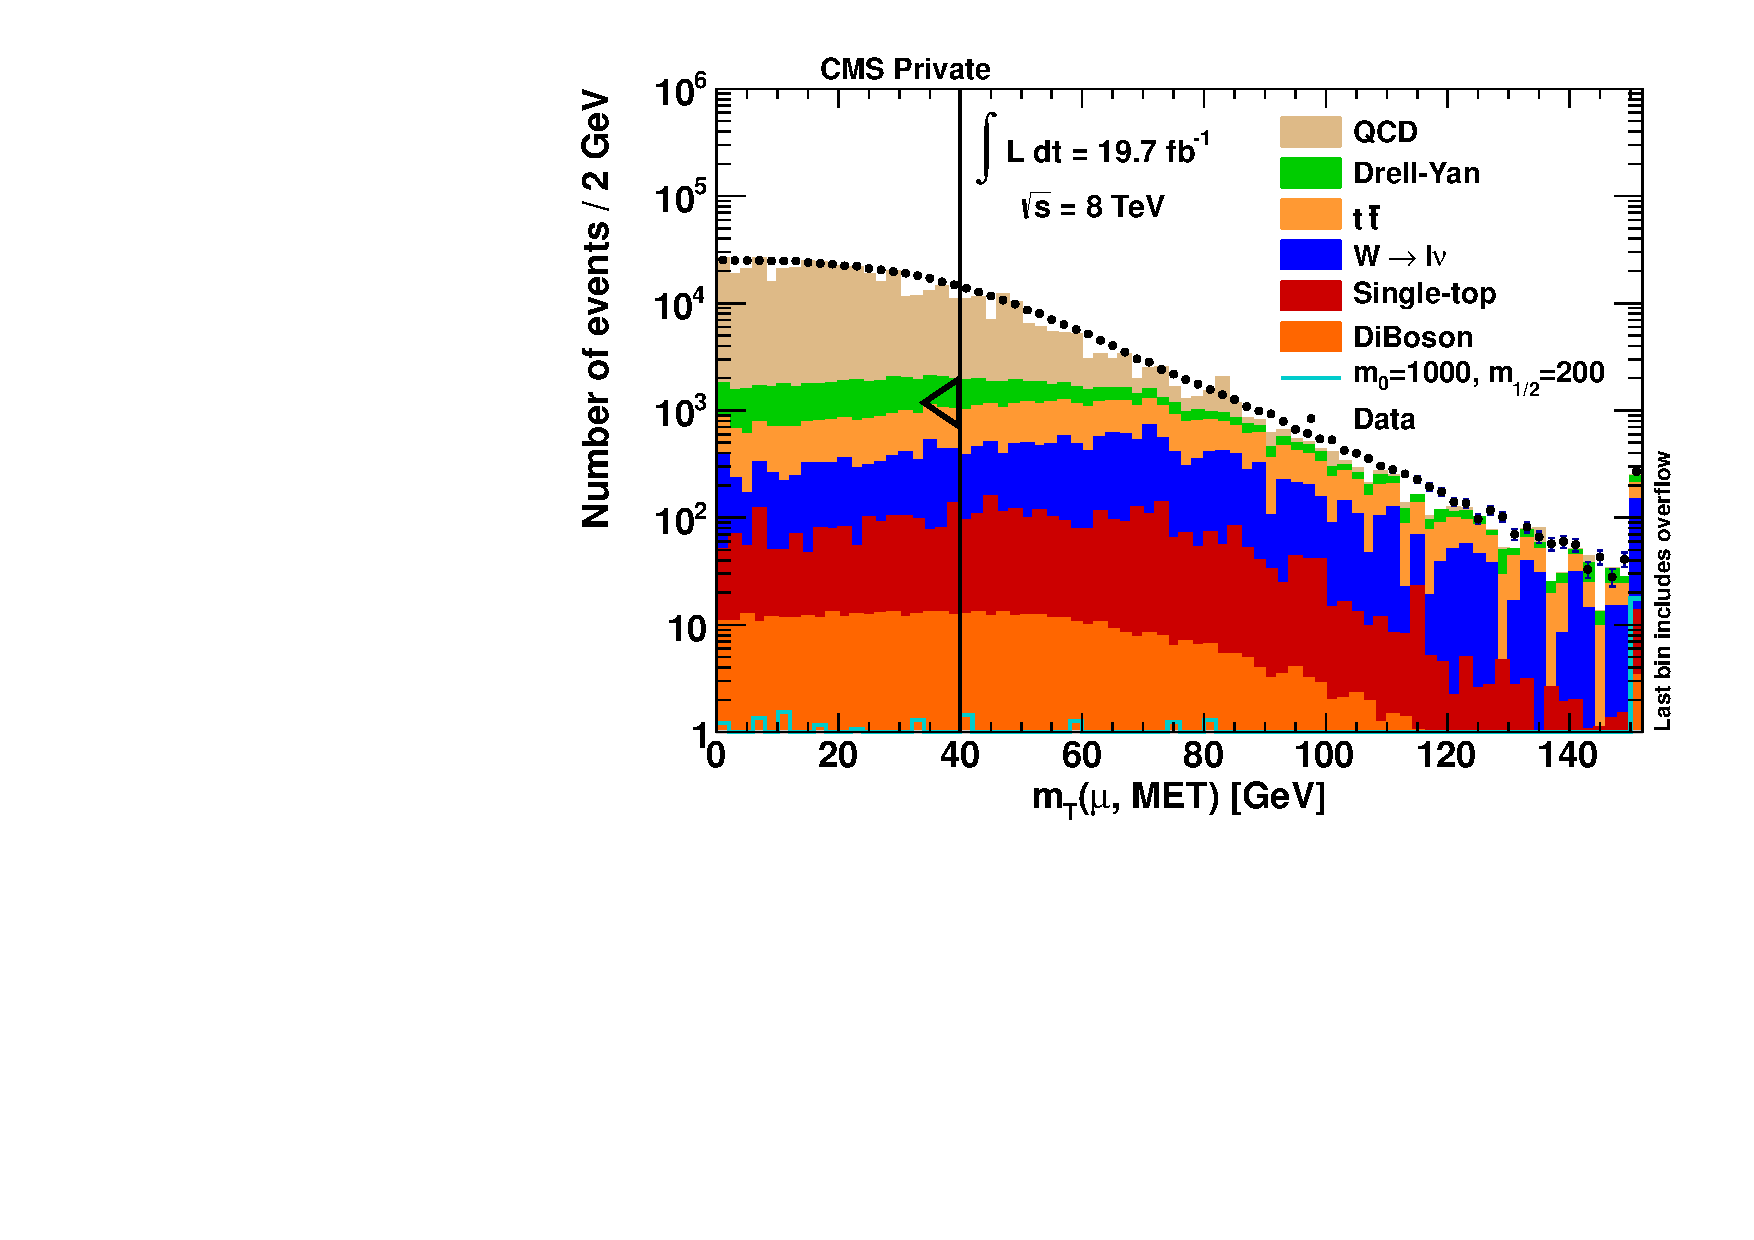
\includegraphics[width=\textwidth]{plots/nTL_mt.pdf}
    \caption{Transverse mass of loose $\mu$ and $E_{\text{T}}^{\text{miss}}$ \label{fig:ntlmt}}
  \end{subfigure}

  \begin{subfigure}[b]{0.495\textwidth}
    \centering
    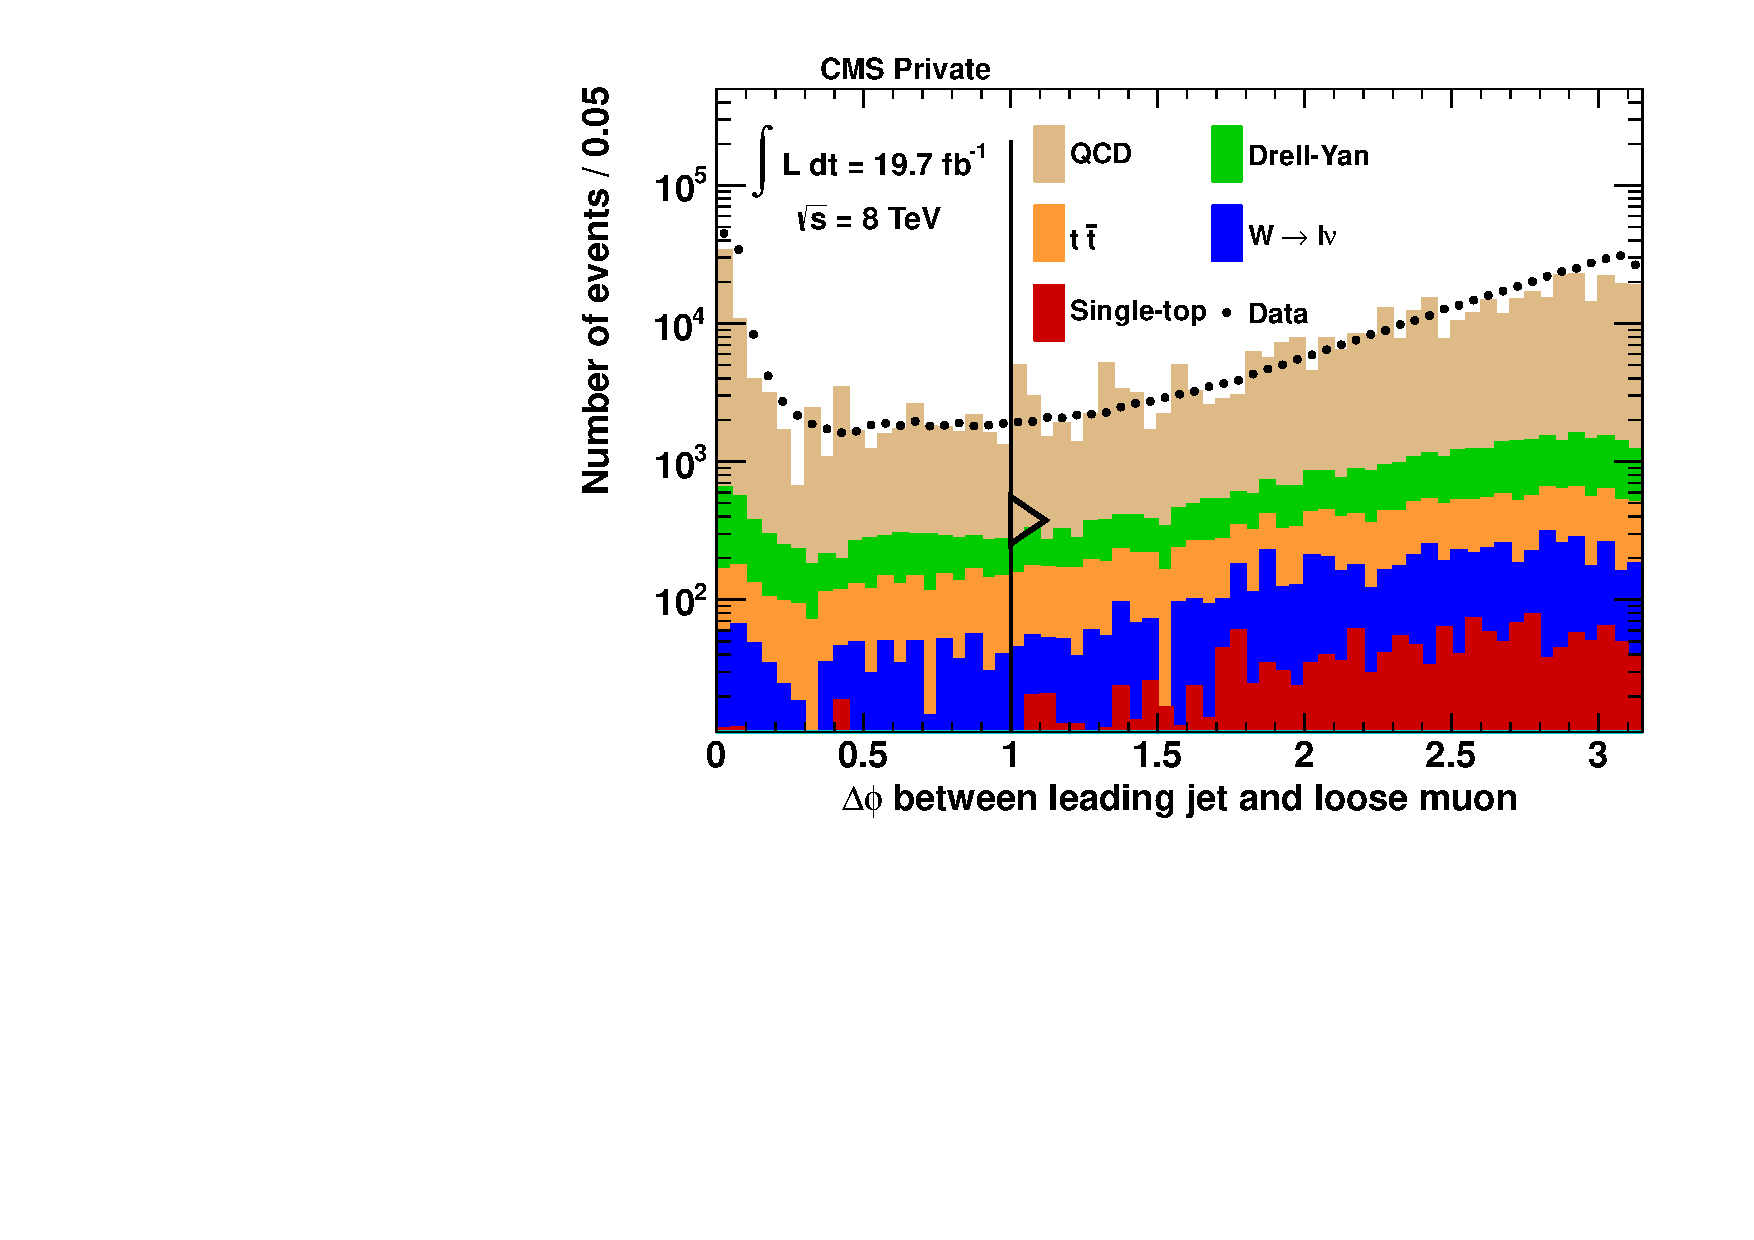
\includegraphics[width=\textwidth]{plots/nTL_jetdphi.pdf}
    \caption{$\Delta \phi$ between loose muon and leading jet \label{fig:ntljetdphi}}
  \end{subfigure}

  \caption{$n - 1$ distributions of the fake rate determiniation. Requirements are indicated by arrows.}
  \label{fig:ntl}
\end{figure}

Counting the number of tight and loose muons in the resulting enriched sample, can be used to predict the hadronic activity leading to possible misidentifications. From the two dimensional tight and loose muon histograms containing the measured data, one has to statistically subtract all background samples. The only exception are the QCD ones, as those are the events this method attempts to predict. The results are shown in figure~\ref{fig:tlratios}.
 
\begin{figure}[!htbp]
  \centering
  \begin{subfigure}[b]{0.495\textwidth}
    \centering
    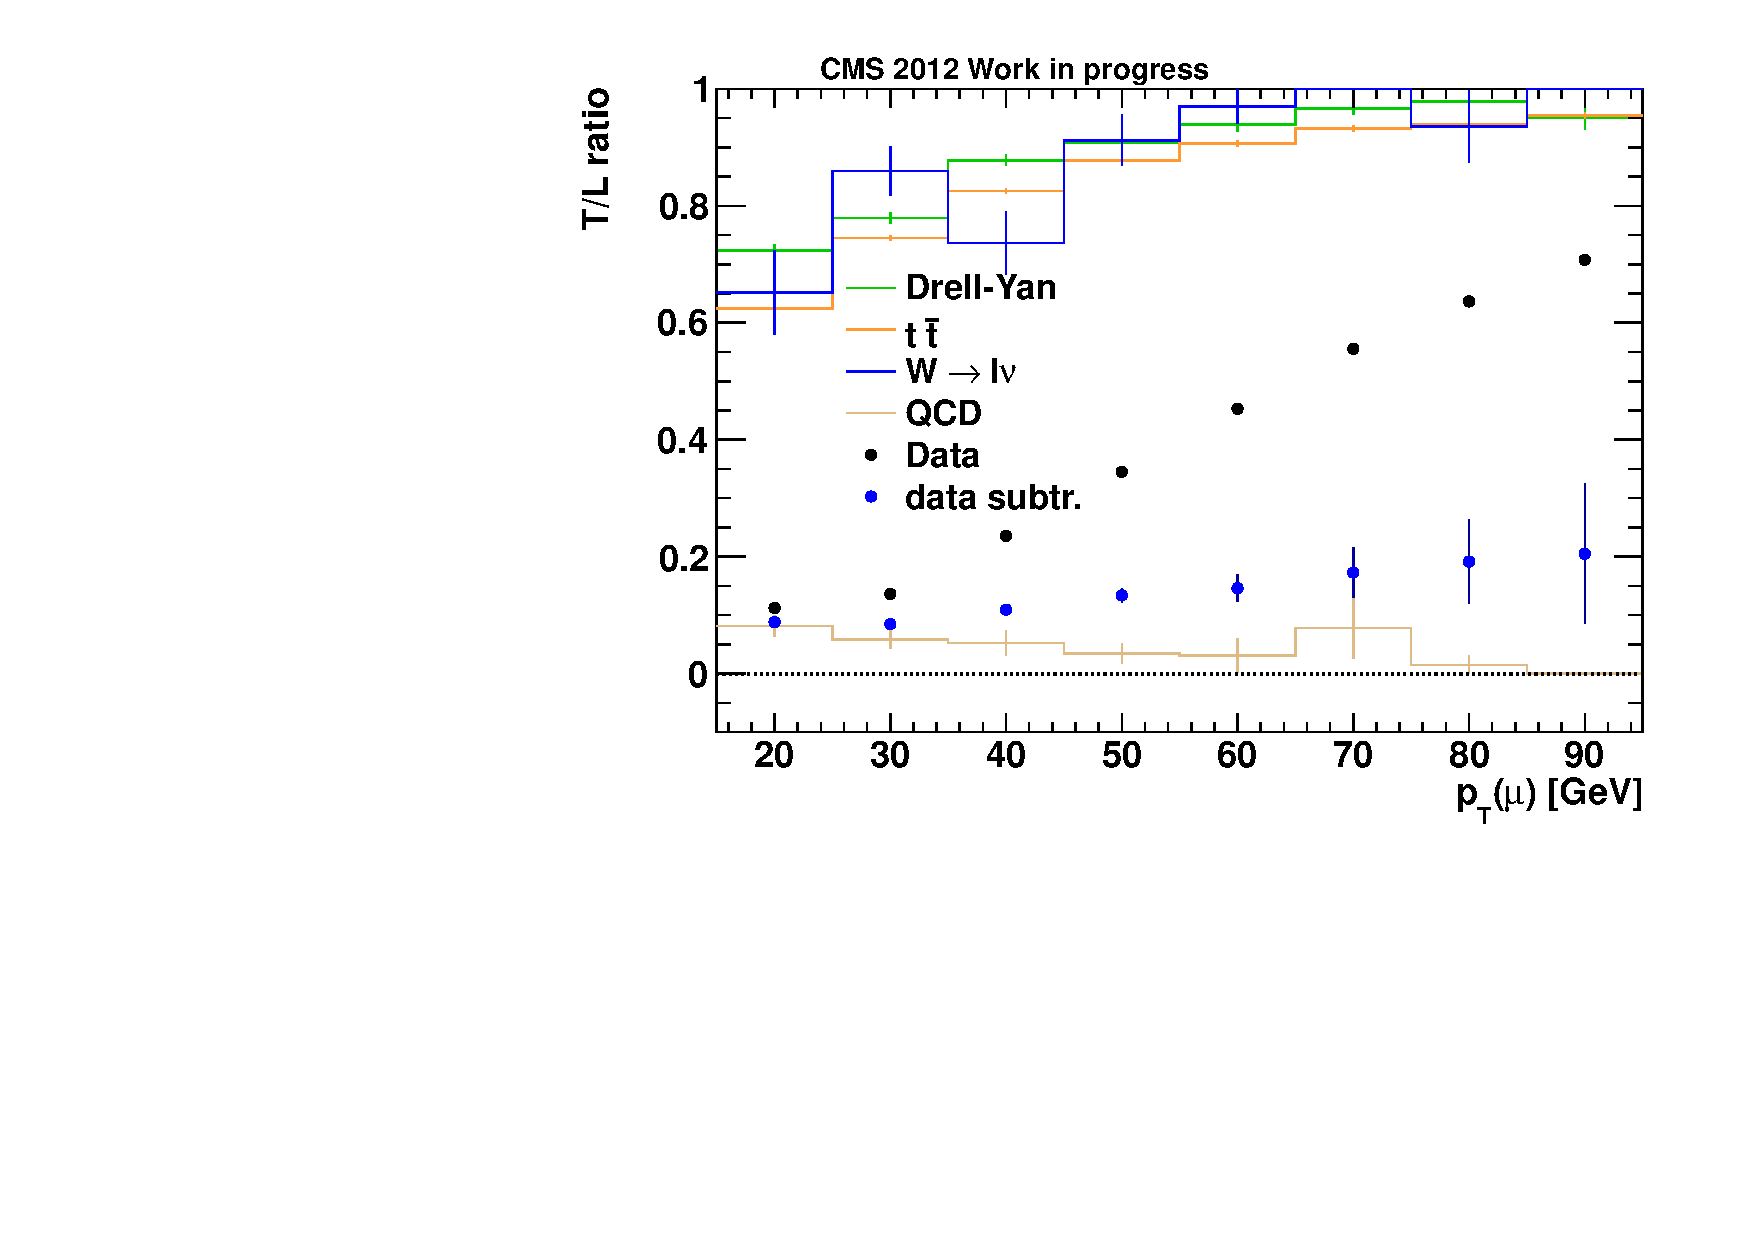
\includegraphics[width=\textwidth]{plots/tlratio.pdf}
    \caption{\label{fig:tlratio}}
  \end{subfigure}
  \begin{subfigure}[b]{0.495\textwidth}
    \centering
    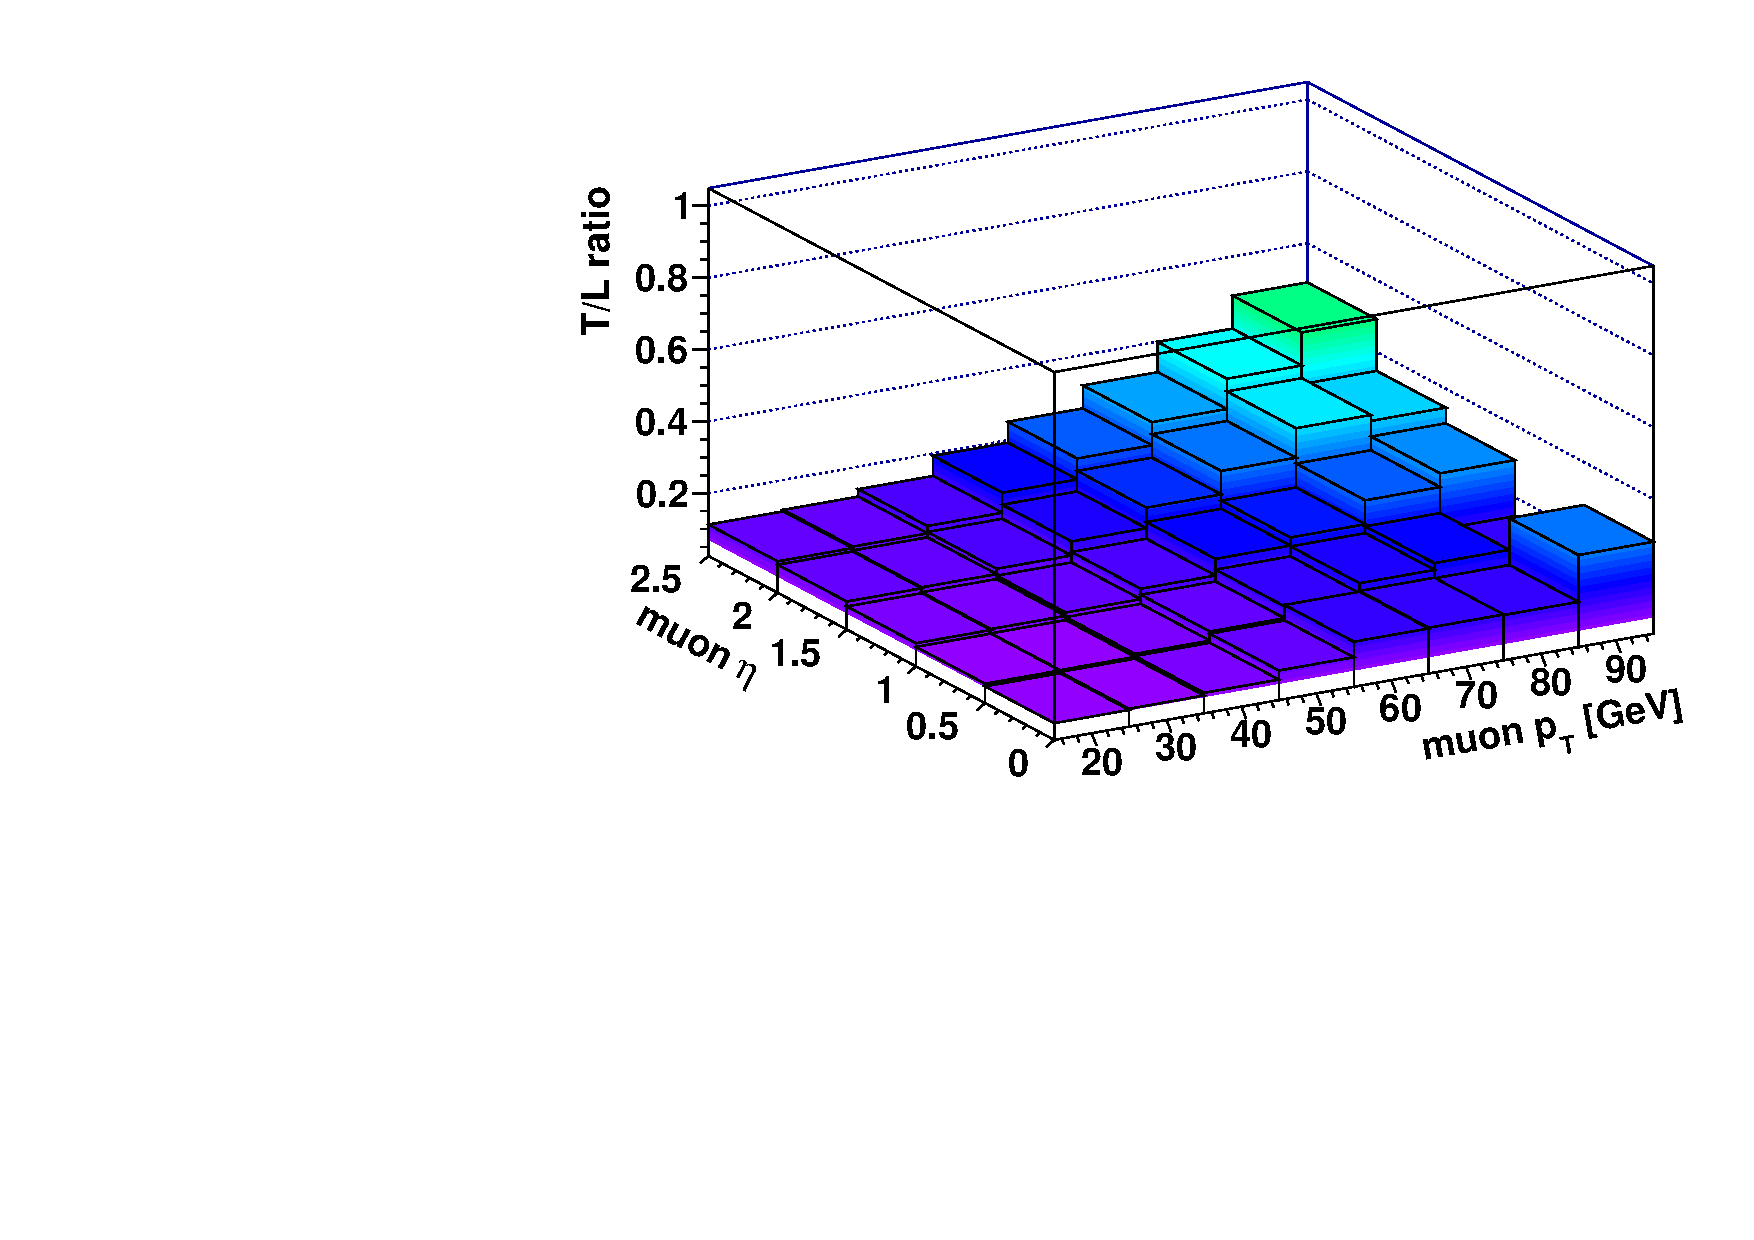
\includegraphics[width=\textwidth]{plots/tlratio2d.pdf}
    \caption{\label{fig:tlratio2d}}
  \end{subfigure}

  \caption{Ratio of tight to loose muons for the calculation of $F_R$. As a function of $p_{\text{T}}$ (\ref{fig:tlratio}) and as a function of both $p_{\text{T}}$ and $\eta$ (\ref{fig:tlratio2d}).}
  \label{fig:tlratios}
\end{figure}

The one dimensional version visualizes various tight-to-loose ratios as a function of $p_{\text{T}}$. While the prediction is depicted by the data points, from which the backgrounds have been subtracted, additional exemplary Monte Carlo samples show the general evolution of the hadronic activity for a few selected backgrounds. Once again, the decreasing statistics towards higher energies and leading order QCD cross sections have to be kept in mind. As the data-driven estimate is meant to describe QCD multijet events, comparing the evolutions of the respective entries reveals that the data behaves differently than expected. Multiple variations of the method's requirements show that the shape of this evolution remains almost identical. This difference has to be kept in mind when determining the uncertainties of this procedure (Sec.~\ref{sec:closure-test}).  

For the actual prediction, $F_R$ is used as a function of $p_{\text{T}}$ and $\eta$ (Fig~\ref{fig:tlratio2d}). Here, the smoothing algorithm that has been introduced in the $b$-tagging section (Sec.~\ref{sec:bjets}), has been employed once more. This allows one to avoid rogue values in bins with a low amount of entries. Should any muon exceed the maximum transverse momentum for which this histogram can provide a reasonable estimate, the value of the corresponding last bin is being used.

\section{Prediction}
\label{sec:tlprediction}

With the tight-to-loose ratio $F_R$ determined, the analysis can be rerun to determine the background estimate. As mentioned in section~\ref{sec:fakerate}, the selection process of the two muons (Sec.~\ref{sec:muonqualy}) has to be altered to be working on an orthogonal sample. Instead of demanding the two tight leptons, one or both of them are replace by loose muons, which are not tight ones. In combination with the respective event weights, this yields single- and double-fake estimates. Figure~\ref{fig:fakeestimates} shows the distributions for both estimates.

\begin{figure}[!htbp]
  \centering
  \begin{subfigure}[b]{0.495\textwidth}
    \centering
    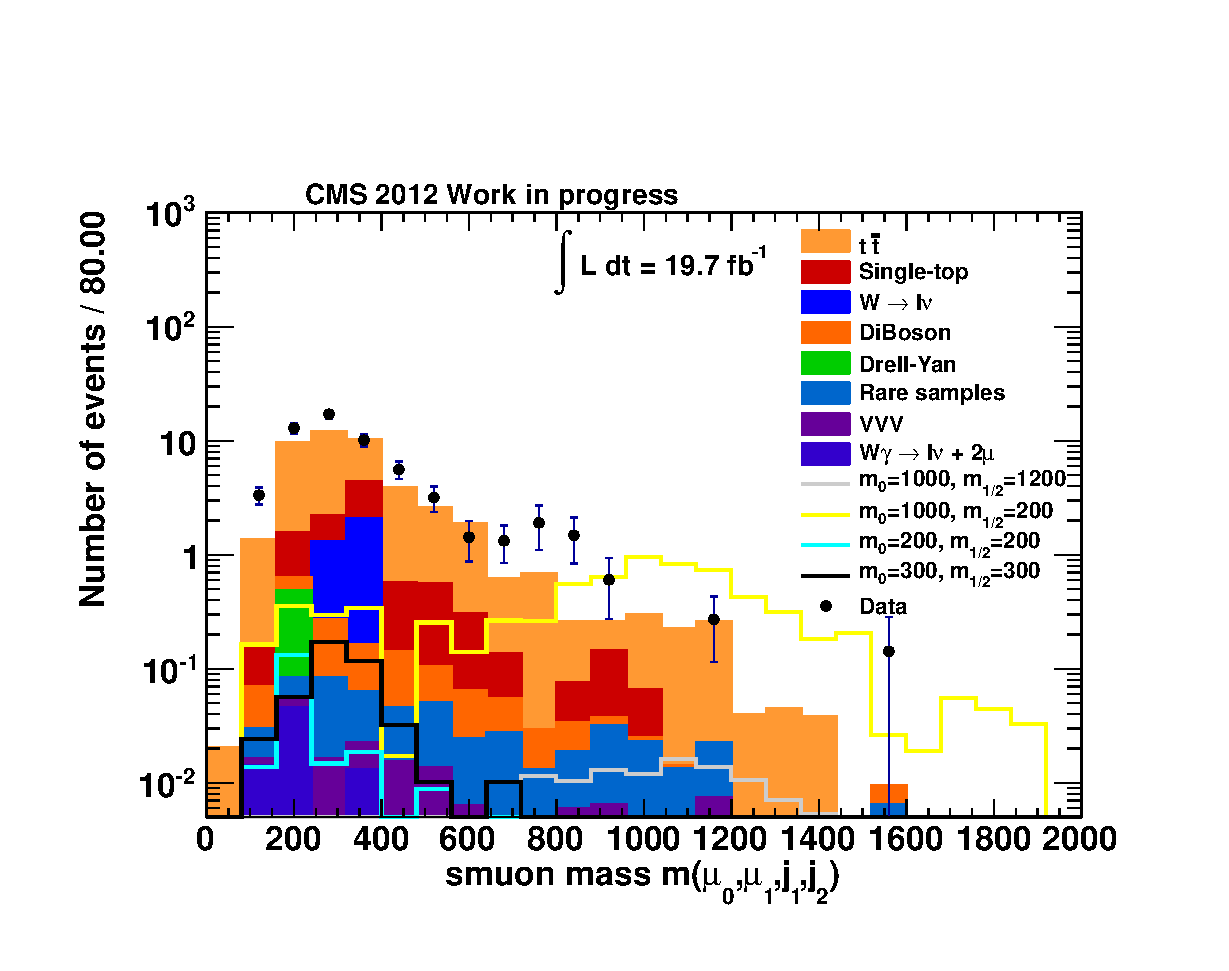
\includegraphics[width=\textwidth]{plots/CR6_m_smuon_singlefake.pdf}
    \caption{\label{fig:CRBVC_m_smuon_singlefake}}
  \end{subfigure}
  \begin{subfigure}[b]{0.495\textwidth}
    \centering
    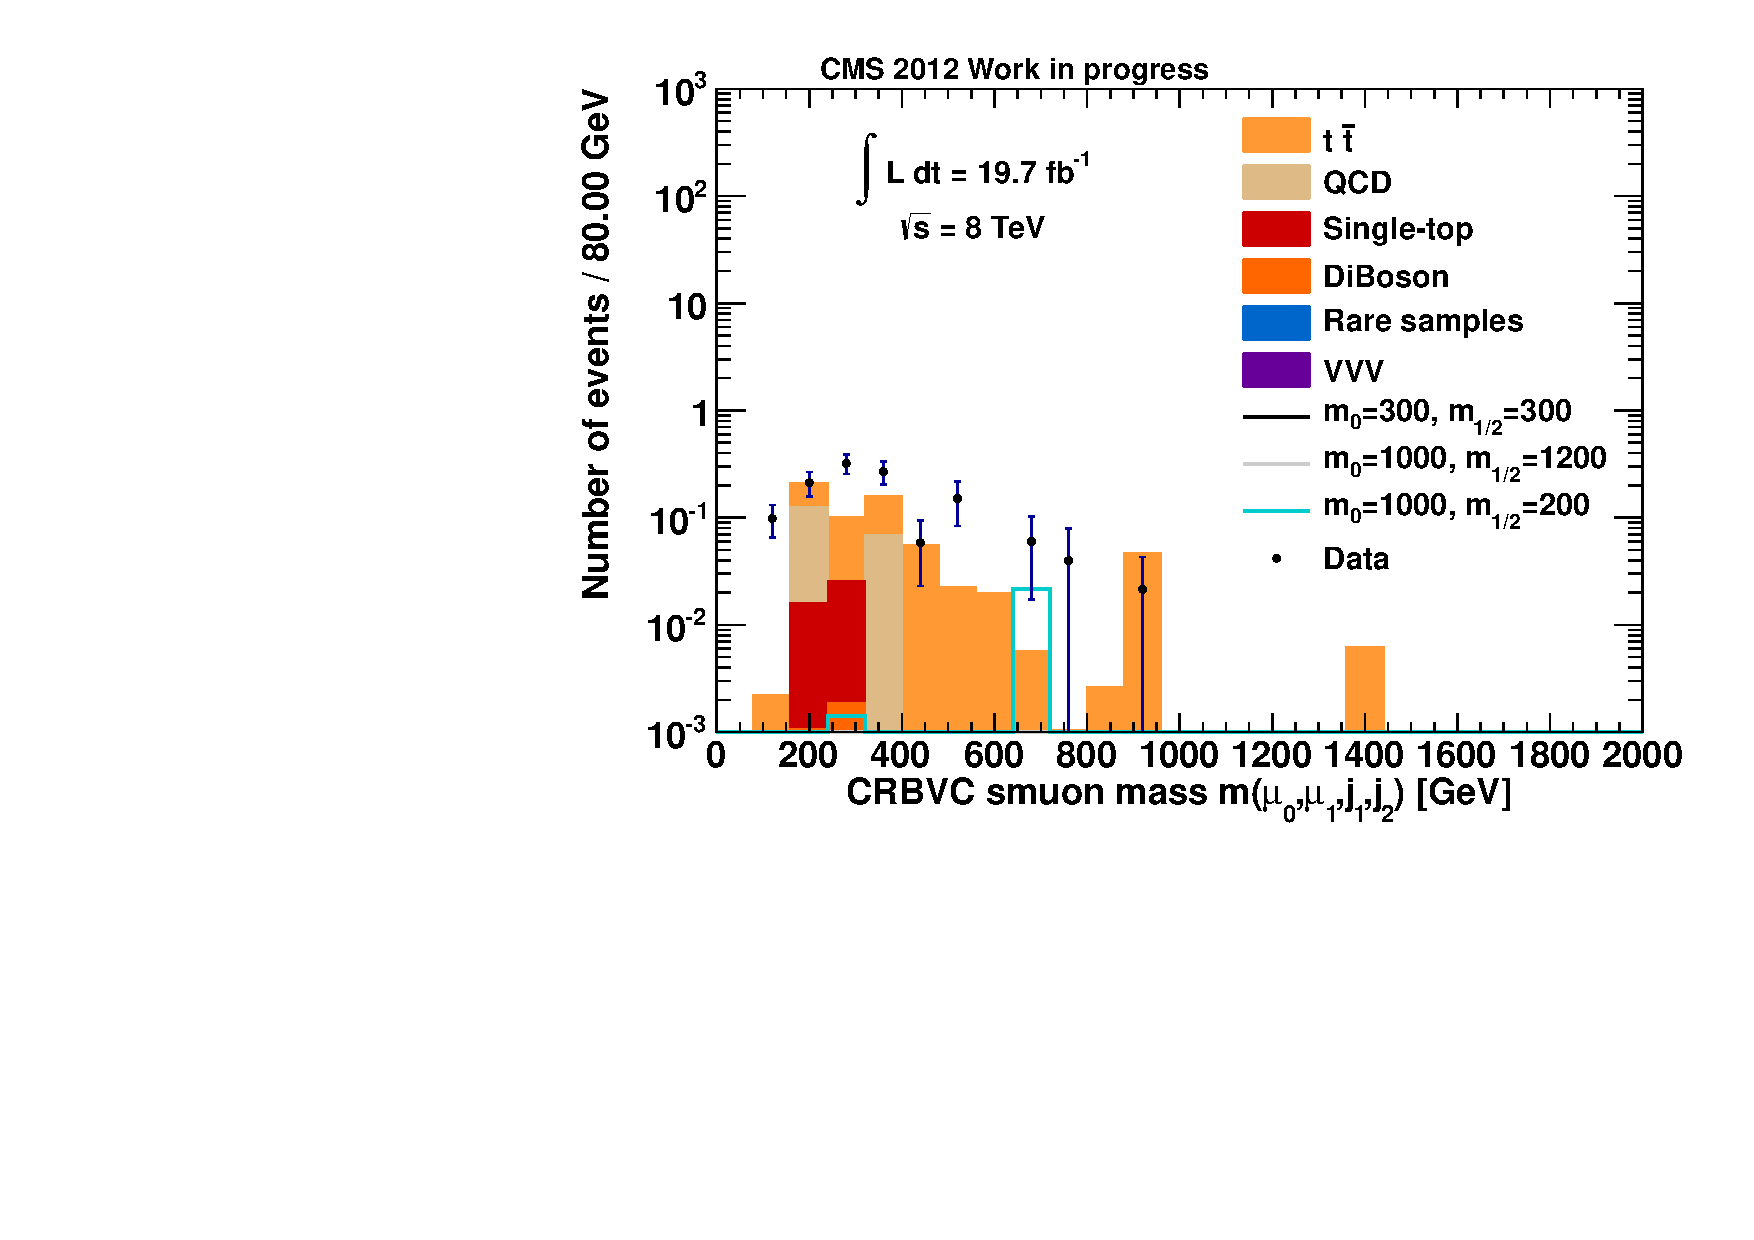
\includegraphics[width=\textwidth]{plots/CR6_m_smuon_doublefake.pdf}
    \caption{\label{fig:CRBVC_m_smuon_doublefake}}
  \end{subfigure}

  \caption{Single- (\ref{fig:CRBVC_m_smuon_singlefake}) and double-fake estimate (\ref{fig:CRBVC_m_smuon_doublefake}) for BVC control region. The latter can be seen before the fake estimate in figure~\ref{fig:ssccr_nofakes}.}
  \label{fig:fakeestimates}
\end{figure}

One can see that the data exceeds the background. This supports the hypothesis, that the contribution of fake muons has an influence on the final state in question. Re-examining the BVC control region previously discussed in section~\ref{sec:sscmuons}, yields the distributions shown in figure~\ref{fig:CRBVC}.

\begin{figure}[hb!]
  \centering
  \begin{subfigure}[b]{0.495\textwidth}
    \centering
    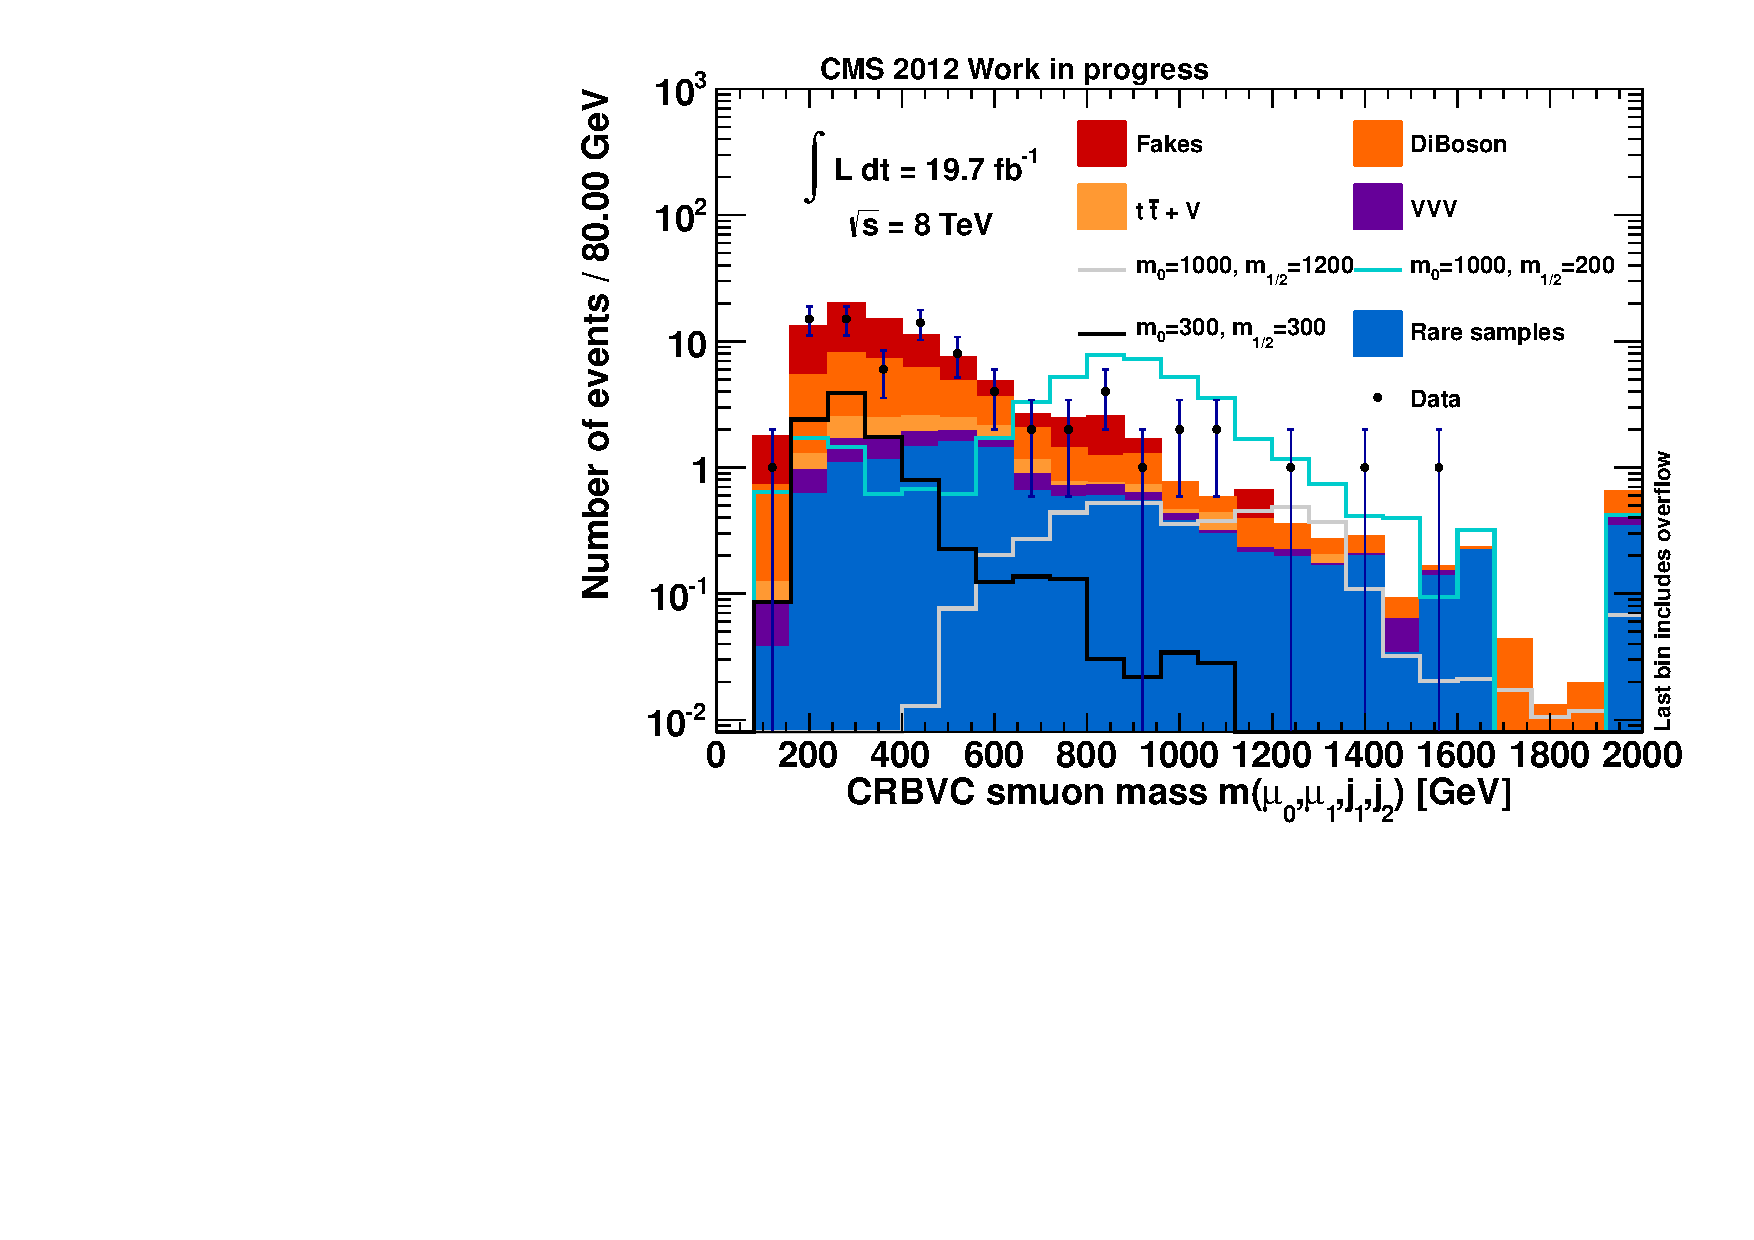
\includegraphics[width=\textwidth]{plots/CR6_m_smuon.pdf}
    \caption{\label{fig:CRBVC_m_smuon}}
  \end{subfigure}
  \begin{subfigure}[b]{0.495\textwidth}
    \centering
    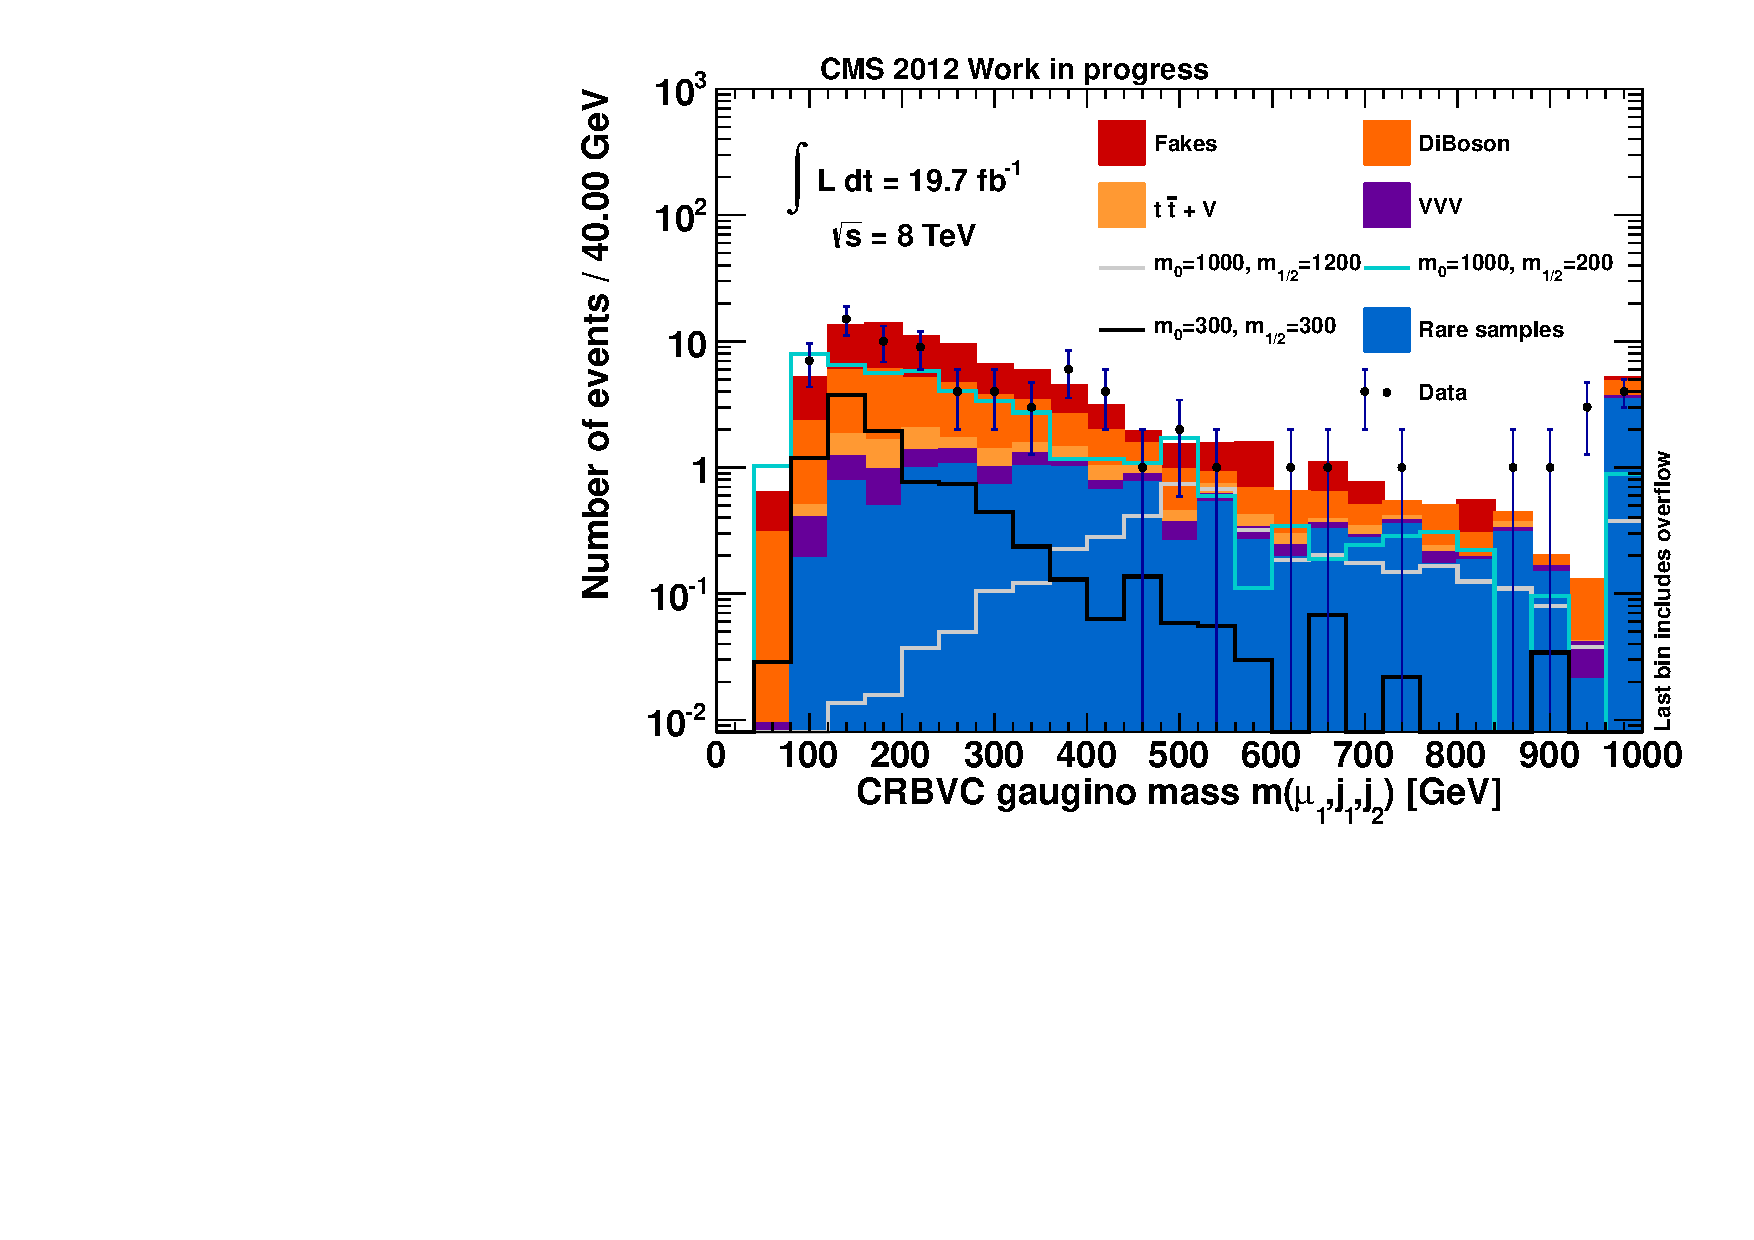
\includegraphics[width=\textwidth]{plots/CR6_m_gaugino.pdf}
    \caption{\label{fig:CRBVC_m_gaugino}}
  \end{subfigure}

  \caption{Smuon mass and gaugino mass of the control region BVC, including the data-driven background estimate.}
  \label{fig:CRBVC}
\end{figure}

With the inclusion of the fake rate method's prediction, the background describes the data significantly better. For a simple quantification of this statement, one can regard the entire distribution as a single bin and compare the number of entries. This yields the following values for the smuon mass distribution: $N_{\text{MC}} = 82.9 \pm 3.6\,(\text{stat.})$ and $N_{\text{Data}} = 75$. A $-0.8\,\sigma$ deviation, purely based off of the Poisson and statistical uncertainty, is a strong indication for the quality of this entire method.


%%% Local Variables: 
%%% mode: latex
%%% TeX-master: "document"
%%% End: 
